%------------------------------------------------------------------------------
% Plantilla Tesis Maestria
%------------------------------------------------------------------------------

\documentclass[11pt,letterpaper,oneside]{book}
\usepackage[activeacute,spanish]{babel}                                         % Lenguaje de la plantilla.
\usepackage[utf8]{inputenc} 			                                        % Español
\usepackage{ucs}
\usepackage[T1,OT1]{fontenc}                                                    % Fuentes de texto.
%\usepackage{libertine}
\usepackage{latexsym}
\usepackage{amsfonts,amsmath,amssymb}                                           % Simbolo AMS.
\usepackage{graphics,graphicx,rotate,epsfig,color}                              % Grafica.
\usepackage{bibunits}                                                           % Bibliografía.
\usepackage{multirow, array}                                                    % Arreglos y multirenglón.
\usepackage{longtable,multirow,booktabs}
\usepackage[x11names,table]{xcolor}
\usepackage[absolute]{textpos}                                                  % Posición del texto.
\usepackage{pstricks,pst-node,amsopn,subfigure}                                 % Figura flotantes.
\usepackage{IEEEtrantools}                                                      % Herramientas IEEE.
\usepackage{fancyhdr,programs}                                                  % Plantilla fancy y programs.
\usepackage{hhline}                                                             % Separación de columnas.
\usepackage{hyperref}
\usepackage{amsmath,amssymb,amsfonts,latexsym,cancel}
\usepackage{mathtools}
\usepackage{url}
\usepackage{hyperref}
\usepackage{float}
\usepackage[justification=centering]{caption}
\usepackage{graphicx}
\usepackage{float}
\usepackage{algorithm}
%\usepackage{algorithmic}
\usepackage{algpseudocode}
\usepackage{subcaption}
\usepackage{subfigure}
\usepackage{colortbl} % Para colorear celdas de tablas
\usepackage{xcolor}
\usepackage{pifont} % Para usar simbolos especiales
\usepackage{tabularx} % Para formatear tablas
\spanishdecimal{.}

%%%%%%%%%%%%%%%%%%%%%%%     Nuevos comandos     %%%%%%%%%%%%%%%%%%%%%%%
\newcommand{\mRx}{\mathbf{R}_\mathbf{x}}
\newcommand{\vrx}{\mathbf{r}_\mathbf{x}}
\newcommand{\mathBF}[1]{\mbox{\boldmath $#1$}}
\newcommand{\V}[1]{\mathBF{#1}}
\newcommand{\M}[1]{\mathBF{#1}}
\newcommand{\cmark}{\ding{51}} % Checkmark
\newcommand{\xmark}{\ding{55}} % Crossmark

%%%%%%%%%%%%%%%%%%%%%%%     Definición de directorios de trabajo     %%%%%%%%%%%%%%%%%%%%%%%
\newcommand{\DirFigP}{./Figures/Portada}
\newcommand{\DirFigCuno}{./Figures/Capitulo1}
\newcommand{\DirFigCdos}{./Figures/Capitulo2}
\newcommand{\DirFigCtres}{./Figures/Capitulo3}
\newcommand{\DirFigCcuatro}{./Figures/Capitulo4}
\newcommand{\DirFigCcinco}{./Figures/Capitulo5}

%%%%%%%%%%%%%%%%%%%%%%%     Datos personales     %%%%%%%%%%%%%%%%%%%%%%%
\title{\Huge \textsc{Desarrollo de un asistente virtual por reentrenamiento de LLMs con recuperación-generación aumentada desde documentos normativos}}     % Titulo del documento.
\author{\LARGE \textit{Ing. Roberto García Guzmán}}                                                                       % Autor del documento.
\date{Diciembre, 2025}                                                                                                % Fecha de publicación.

%%%%%%%%%%%%%%%%%%%%%%%     Archivos incluidos     %%%%%%%%%%%%%%%%%%%%%%%%%%%%%%%
%  Archivos de tesis
\includeonly{portada}

%  Capítulos
\includeonly{Capitulo1,Capitulo2,Capitulo3,Capitulo4,Conclusiones}
\hyphenation{}

%%%%%%%%%%%%%%%%%%%%%%%     Inicio del documento     %%%%%%%%%%%%%%%%%%%%%%%
\begin{document}

\renewcommand{\tablename}{Tabla}                                                % Cambiar la palabra "Cuadro" por "Tabla"
%\renewcommand{\listtablename}{Índice de Tablas}
\thispagestyle{empty}
\textblockorigin{0mm}{0mm}
\pagestyle{empty}

\begin{textblock}{6}(1.1,1.1)    %1.05, 1.2
    \includegraphics[width=4.3cm]{\DirFigP/escudo-bn}
\end{textblock}

\begin{textblock}{10}(4.5,1.8)
    \begin{center}
        \huge{UNIVERSIDAD DE GUANAJUATO}
    \end{center}
\end{textblock}

\begin{textblock}{10}(4.8,2.23)
    \begin{flushleft}
        \rule{13cm}{0.5mm}
    \end{flushleft}
\end{textblock}

\begin{textblock}{10}(4.8,2.3)
    \begin{flushleft}
        \rule{13cm}{1.0mm}
    \end{flushleft}
\end{textblock}

\begin{textblock}{10}(4.8,2.4)
    \begin{flushleft}
        \rule{13cm}{0.5mm}
    \end{flushleft}
\end{textblock}

\begin{picture}(0,0)
    \thicklines

    \put(-48,-60){\line(0,-1){530}} \put(-47,-60){\line(0,-1){530}}
    \put(-46,-60){\line(0,-1){530}} \put(-45,-60){\line(0,-1){530}}

    \put(-25,-65){\line(0,-1){535}} \put(-24,-65){\line(0,-1){535}}
    \put(-23,-65){\line(0,-1){535}} \put(-22,-65){\line(0,-1){535}}

    \put(-2,-60){\line(0,-1){530}} \put(-3,-60){\line(0,-1){530}}
    \put(-4,-60){\line(0,-1){530}} \put(-5,-60){\line(0,-1){530}}
\end{picture}

\begin{textblock}{10}(4.5,2.7)
    \begin{center}\Large{CAMPUS IRAPUATO-SALAMANCA\\DIVISIÓN DE INGENIERÍAS}
    \end{center}
\end{textblock}

\begin{textblock}{10}(4.6,4.5)
    \begin{center} \LARGE {\textit{Desarrollo de un asistente virtual por reentrenamiento de LLMs con recuperación-generación aumentada desde documentos normativos}}
    \end{center}
\end{textblock}

\begin{textblock}{12}(3.45,7.0)
    \begin{center} \huge{\bf{TESIS}} \end{center}
\end{textblock}

\begin{textblock}{12}(3.45,8.5)
    \begin{center} \small{\bf{ QUE PARA OBTENER EL TÍTULO DE:}} \end{center}
\end{textblock}

\begin{textblock}{12}(3.45,8.9)
    \begin{center} \emph {MAESTRO EN INGENIERÍA ELÉCTRICA} \end{center}
\end{textblock}

\begin{textblock}{12}(3.6,10.1)
    \begin{center} PRESENTA: \end{center}
\end{textblock}

\begin{textblock}{12}(3.45,10.6)
    \begin{center} \Large{\textit{\textbf{Ing. Roberto García Guzmán}}} \end{center}
\end{textblock}

\begin{textblock}{12}(3.45,12.0)
    \begin{center} DIRECTORES: \end{center}
\end{textblock}

\begin{textblock}{12}(3.45,12.4)
    \begin{center} \large\textit{Dra. Dora Luz Almanza Ojeda}  \end{center}
\end{textblock}

\begin{textblock}{12}(3.45,12.8)
    \begin{center} \large\textit{Dr. Yair Alejandro Andrade Ambriz}  \end{center}
\end{textblock}

\begin{textblock}{9.5}(4.6,14.7)
    \begin{center} SALAMANCA, GTO. \hspace{1.8in} Diciembre, 2025 \end{center}
\end{textblock}

%\begin{textblock}{100}(1.95,4.8)
%\includegraphics[scale=1]{\DirFigP/Porta.eps}
%\end{textblock}

\begin{picture}(0,0)
    \thicklines
\end{picture}

\newpage
                                                      % Portada
\pagestyle{fancy}                                                               % Estilo de página
\fancyhead{}                                                                    % Encabezado de la página
% Aquí se fija el formato de la página
%\paperwidth     =   +8.50in % Ancho del papel
%\paperheight    =   +11.00in% Largo del papel
% Vertical
\voffset        =   +0.00in % Espacio vertical en la página sobre una pulgada

\topmargin      =   -0.40in % Separación entre encabezado y margen
%\headheight     =   +0.25in % Ancho del encabezado
\headheight     =   +0.30in % Ancho del encabezado
%\headsep        =   +0.25in % Separación entre encabezado y cuerpo
\headsep        =   +0.50in % Separación entre encabezado y cuerpo

\textheight     =   +8.00in % Alto del cuerpo

\footskip       =   +0.50in % Suma de separación de cuerpo y ancho de pie

% Horizontal
\hoffset        =   +0.00in % Espacio horizontal en la página sobre una pulgada
%\oddsidemargin  =   +0.50in % Espacio horizontal en páginas par
%\evensidemargin =   +0.25in % Espacio horizontal en página impar
\evensidemargin =   -0.25in % Espacio horizontal en página impar

%\textwidth      =   +4.50in % Ancho del cuerpo
\textwidth      =   +6.00in % Ancho del cuerpo

\marginparsep   =   +0.00in % Separación entre notas y cuerpo
\marginparwidth =   +0.00in % Ancho de notas

\parskip        =   +0.20in % Espacio en encabezado
\lineskip	=   +0.60in
\linespread{1.2}            % Separación entre líneas
\baselineskip  = +0.23in
                                                       % Diseño de hoja
\pagestyle{fancy}       % Estilo de página fancy
\fancyhead{}            % Encabezado de la página
\addtolength{\headwidth}{\marginparsep}
                        % Incrementa la longitud en el encabezado
\addtolength{\headwidth}{\marginparwidth}
                        % Incrementa la longitud en el encabezado
\renewcommand{\headrulewidth}{0.4pt}
                        % Ancho de la regla del encabezado de página
\renewcommand{\footrulewidth}{0.4pt}
                        % Ancho de la regla del pie de página
\renewcommand{\chaptermark}[1]{\markboth {#1}{#1}}
                        % Marca de nombre de capitulo
\renewcommand{\sectionmark}[1]{\markright {\thesection~#1}}
                        % Marca de nombre y numero de sección
%\lhead[\fancyplain{}{\normalsize\scshape\leftmark}]{\fancyplain{}{\small\scshape\rightmark}}
\renewcommand{\baselinestretch}{1.5}

\lhead[\fancyplain{}{\bfseries\thepage}]{\fancyplain{}{\bfseries\rightmark}}
                        % Margen izquierdo superior capitulo o sección
%\rhead[\fancyplain{}{\slshape\leftmark}]{\fancyplain{}{\slshape\rightmark}}
\rhead[\fancyplain{}{\bfseries\leftmark}]{\fancyplain{}{\bfseries}}
                        % Margen derecho superior número de página
%\cfoot{\thepage}
\cfoot{\thepage}                        % Pie de página central
\chead{}
                        % Encabezado de página central

                                                      % Formato de tesis
\pagenumbering{arabic}                                                          % Tipo de letra
%\onehalfspace
%\chapter*{Agradecimientos Personales}
\vspace{-1cm}

A mis asesores, la Dra. Dora y el Dr. Yair, por guiarme en esta etapa y
darme la oportunidad de desenvolverme con libertad.

A mis nuevos amigos, Jessica y Alejandro, que me acompañaron durante esta
etapa y me permitieron compartir con ellos muchas experiencias.

A mi familia, por su apoyo incondicional.

A mi esposa, Isis, por su amor, paciencia y apoyo ilimitados, sin tí
no hubiera sido posible.                                             % Agradecimientos
%\chapter*{Agradecimientos Institucionales}
\vspace{-1cm}

A la Universidad de Guanajuato, División de Ingenierías del Campus
Irapuato-Salamanca (DICIS) por brindarme la formación académica y la
infraestructura que me permitió llevar a cabo mis estudios.

\begin{figure}[h]
    \centering
    \includegraphics[width=0.8\textwidth]{\DirFigP/ingenierias}
\end{figure}

A la Secretaría de Ciencia, Humanidades, Tecnología e Innovación, SECIHTI
de México, por el apoyo económico otorgado a bajo el CVU \textbf{2006734}.

\begin{figure}[h]
    \centering
    \includegraphics[width=0.8\textwidth]{\DirFigP/secihti}
\end{figure}

\tableofcontents                                                               % Índice general
%\listoffigures

% Índice de figuras
%\listoftables                                                                  % Índice de tablas
%\chapter{Resumen}

Los documentos normativos son un componente fundamental de las organizaciones,
las cuales tienen la responsabilidad de difundirlos y lograr que sus miembros
los comprendan. Para facilitar esta labor, es posible emplear tecnologías de
cómputo modernas y técnicas de procesamiento de lenguaje natural con el fin
de generar sistemas inteligentes que faciliten la consulta y compresnsión
de la normativa.

En este trabajo se presenta un asistente virtual, basado en LLMs de código
abierto y técnicas de Recuperación-Generación Aumentada (RAG, Retreival-Augmented
Generation), diseñado para responder preguntas sobre la normativa de la
Universidad de Guanajuato utilizando como única fuente de información los
documentos oficiales disponibles en formato PDF. El sistema alcanzó una
puntuación BERT de 0.75 y un porcentaje de aciertos del 88\%. Una primera
contribución de este trabajo es la implementación de un asistente capaz
de ofrecer respuestas referenciadas, vinculando cada salida con los artículos
y documentos correspondientes.

La segunda contribución consiste en el desarrollo de una metodología de
extracción de información a partir de documentos PDF, la cual aprovecha sus
elementos visuales para recuperar la estructura jerárquica de la normativa.
Esto facilita la separación en fragmentos y permite relacionar correctamente
cada respuesta con los artículos correspondientes de los documentos
oficiales. Para la recuperación de información y la generación de respuesta,
se evaluaron distintos modelos de extracción de \textit{embeddings} y de
inferencia, seleccionando los más aptos considerando su desempeño
y el hardware disponible: Qwen3-Embedding-8B-Q4\_K\_M como extractor de
\textit{embeddings} y gpt-oss-20b-MXFP4 para la inferencia.

Además, se generó un conjunto de preguntas y respuestas basadas en la
normativa de la Universidad de Guanajuato con el fin de evaluar los modelos
y reentrenar dos extractores de \textit{embeddings} mediante el ajuste
completo de sus parámetros. Uno de estos modelos alcanzó un recall de 0.88,
lo que, si bien es inferior al 0.93 del modelo óptimo, muestra que es
posible mejorar el desempeño de los modelos base mediante reentrenamiento
con los datos obtenidos.

Finalmente, la tercera contribución es la implementación de una arquitectura
de nube híbrida para poner el sistema en producción, aprovechando los
recursos locales de la institución y permitiendo el acceso a través de
una aplicación web por la cual los usuarios interactúan con los modelos de
lenguaje.
		                                                % Prologo
\newpage

%%%%%%%%%%%%%%%%%%%%%%%     Capítulos     %%%%%%%%%%%%%%%%%%%%%%%

%\pagenumbering{arabic}
\chapter{Introducción}

Todas las organizaciones requieren un conjunto de normas para funcionar adecuadamente.
Si bien, en algunas organizaciones, las normas se dan a conocer de forma verbal,
las organizaciones constituidas formalmente requieren que sus lineamientos se encuentren
redactados en documentos para evitar errores o ambigüedades en la
aplicación de los mismos.

En organizaciones grandes, los documentos normativos suelen ser extensos y poseer un
lenguaje que no es familiar para todos los miembros, lo cual puede dificultar el
entendimiento completo de las normas.

Por otro lado, en la última década, se han presentado avances significativos
en lo que popularmente se conoce como \textit{Inteligencia Artificial}, tratándose
específicamente de una mejora notable en los modelos de lenguaje, que ahora
permiten a los sistemas computacionales comunicarse con los usuarios empleando
lenguaje natural y desempeñar tareas relacionadas con la interpretación de texto.

Con el objetivo de aprovechar estas herramientas y favorecer a la comunidad
universitaria, surge el propósito de proveer una herramienta que ayude a conocer
y entender la normativa de la Universidad de Guanajuato. Para ello, se emplearán
técnicas modernas de procesamiento de texto para crear un asistente virtual,
tipo chatbot, que tenga la capacidad de resolver dudas acerca de la los
documentos normativos de la universidad de forma fundamentada, y así, evitar
la vulneración de los derechos de la comunidad y evitar omisiones en el
cumplimiento de sus obligaciones.

\section{Justificación}

La normatividad vigente de la Universidad de Guanajuato (UG) se puede consultar
en su página oficial \footnote{https://www.ugto.mx/}, en la cual se presentan
22 documentos de solo texto en formato PDF que, en conjunto, pesan 6.9 MB. Si
se convierten estos documentos a texto plano, se obtienen 1.1 MB de información,
lo que equivale a 168,011 palabras. Además, la página web presenta otros documentos
relevantes como el Plan de Desarrollo Institucional, la Gaceta Universitaria,
entre otros, los cuales abonan a la cantidad de textos que se espera que
alumnos, docentes y administrativos conozcan y den seguimiento a sus actualizaciones.

Sin embargo, una dificultad que se presenta al momento de divulgar documentos de carácter
oficial es la falta de cultura lectora en la sociedad mexicana. Según
datos del MOLEC 2024 (Módulo de lectura del INEGI) \cite{inegi_modulo_2024},
el porcentaje de población lectora disminuyó 14.6 puntos porcentuales en los últimos
nueve años, pasando del 84.2 \% en 2015 al 69.6 \% en 2024. Aunque se observa
una leve mejora de la cantidad de población lectora con respecto a 2023 (68.5 \%),
la falta de hábitos de lectura en la población es notable. De aquí se
presenta la necesidad de proponer estrategias alternativas en la divulgación de documentos
normativos, como puede ser el uso de asistentes inteligentes.

Por otra parte, el Foro Económico Mundial 2020 (WEF) presentó el concepto de
Educación 4.0 \cite{world_economic_forum_schools_2020}, en la cual se reconoce que la
educación debe adaptarse a las necesidades del futuro y para ello el UNESCO-UNEVOC
(Centro internacional para la Educación y Formación Técnica y Profesional)
define la Educación 4.0 como una técnica de aprendizaje que se centra en
transformar la educación con el uso de tecnologías avanzadas, reconociendo la
Inteligencia Artificial como una de ellas. Alineado con esta visión, este proyecto
pretende servir como ejemplo de la integración de la inteligencia artificial en
el ámbito educativo, para resolver una de las necesidades de la comunidad. Así
mismo, ayudará a fomentar el uso responsable de las tecnologías como los chatbots
inteligentes al emplearlos como herramientas de apoyo en la interpretación de
documentos normativos.

Aunado a lo anterior, desde la introducción de ChatGPT en 2022 \cite{openai_introducing_2022},
los modelos de lenguaje con capacidades conversacionales, o chatbots inteligentes,
se han integraron en diversos ámbitos de la vida cotidiana, siendo el ámbito
académico uno de los más influenciados. Estos cambios motivan a los investigadores
a analizar el impacto que tienen estas herramientas en la educación, como es el
caso de Peláez-Sánchez et al. \cite{pelaez-sanchez_impact_2024}.
Así mismo, se introduce la incógnita de los usos se les puede dar a estas herramientas en
beneficio de la comunidad académica, siendo ésta la motivación del presente proyecto.

Si bien en el mercado actual existen chatbots inteligentes que pueden
responder preguntas relacionadas a documentos que les sean proporcionados, es
difícil proporcionarles todo el contexto necesario para que sus respuestas sean
correctas, que provengan de fuentes autorizadas y estén debidamente
referenciadas. Además, estas herramientas comerciales tienen desventajas
marcadas como que suelen estar sujetas a políticas de uso o privacidad que pueden
ser desfavorables para los usuarios, puede haber variaciones
en su costo, el nivel de personalización es limitado y generalmente se desconoce
el uso que se les da a los datos confidenciales que se comparten en ellas. Lo anterior
obliga a considerar opciones de código abierto, con las que se puede alcanzar
un nivel de personalización mayor, mejor control sobre las políticas de privacidad
y garantizar la continuidad del sistema con un plan adecuado de mantenimiento
y actualización. Es bajo esta filosofía que este proyecto pretende crear un sistema
adaptado a las necesidades de los usuarios y que funcione con opciones de código
abierto.

\section{Antecedentes}

El Procesamiento de Lenguaje Natural (NLP, Natural Language Processing) es una rama
de la inteligencia artificial y la lingüística, dedicada a dotar a las computadoras
de entendimiento de frases o  palabras escritas en lenguajes humanos \cite{khurana_natural_2023}.
En este proyecto, intervienen diferenes áreas del NLP, como son el modelado de lenguaje
(LM, Language Modeling), la respuesta a preguntas (QA, Question Answering) y la
similitud semántica de texto (STS, Semantic Textual Similarity), por mencionar
las más importantes.

Respecto al modelado de lenguaje, es el área del NLP que pretende predecir la siguiente palabra o carácter en una
secuencia de texto dada. En las úlitmas décadas, se han presentado avances significativos
como son: el modelo neuronal probabilístico de Bengio et al. \cite{bengio_neural_2003}
que empleaba una red neuronal y una tabla de búsqueda para predecir el siguiente carácter;
el uso de redes neuronales entrenadas de forma semisupervisada para aprendizaje
multitarea propuesto por Collobert \& Weston \cite{collobert_unified_2008}; la
introducción de embeddings para aprender representaciones vectoriales distribuidas
de las palabras por Mikolov et al. \cite{mikolov_distributed_2013};
la aparición de los modelos sequence-to-sequence que empleaban Memoria a
Largo Corto-Plazo (LSTM) para convertir una secuencia de texto en otra por
Sutskever et al \cite{sutskever_sequence_2014}; la mejora de los modelos
codificador-decodificador empleando mecanismos de atención para detectar partes de la
oración que son relevantes por parte de Bahdanau et al. \cite{bahdanau_neural_2016};
y por último, la introducción de los transformers, los cuales
son una arquitectura de red neuronal basada únicamente en mecanismos de atención
\cite{vaswani_attention_2017} que alcanzaron excelentes resultados en tareas de traducción
máquina. Es en este proceso que surgen los Modelos de Lenguaje de Gran Tamaño
(LLM, Large Language Models), los cuales emplean técnicas de aprendizaje profundo,
particularmente arquitecturas basadas en transformers, para aprender y entender
patrones complejos y estructuras presentes en los datos.

Estos avances llevaron a la creación del Transformer Generativamente Preentrenado
(GPT) por Radford et al. \cite{radford_improving_2018}, una arquitectura basada en
transformers, acompañada de método de entrenamiento que consiste en preentrenar un modelo de
lenguaje para predecir la siguiente palabra, empleando un corpus de texto sin
etiquetar, seguido de un ajuste fino en tareas específicas. Con esta técnica,
fue posible alcanzar resultados superiores al estado del arte en
diversas tareas de NLP, como son la inferencia de lenguaje natural,
dar respuesta a preguntas, búsquedas por similitud semántica, entre otras.

La presentación del modelo GPT fue seguida de mejoras que incluyeron conjuntos de
entrenamiento más extensos, cambios en las técnicas de ajuste fino, incremento en
el tamaño del modelo, entre otras, dando como resultado el lanzamiento de
ChatGPT-3 \cite{openai_introducing_2022}, definido como un modelo que interactúa de forma
conversacional con capacidad de responder preguntas de seguimiento, admitir sus
errores, objetar premisas incorrectas y rechazar peticiones inapropiadas. Tras
la liberación de ChatGPT-3 al público, múltiples empresas y organizaciones han
empleado metodologías de entrenamiento similares para desarrollar sus propios
modelos conversacionales y competir en el mercado.

Estos modelos conversacionales caen en la categoría de chatbots, los cuales se
definen como sistemas computacionales inteligentes con capacidades de conversación,
que son diseñados para emular una conversación humana con el objetivo de
proporcionar orientación o apoyo \cite{caldarini_literature_2022}.

En la actualidad, los modelos generativos basados en transformers como Chat GPT-4
(OpenAI), Gemini (Google), Llama (Meta), DeepSeek (DeepSeek), entre otros, son el
estado del arte en cuanto a chatbots multidominio, ya que pueden responder preguntas
y realizar tareas en diferentes dominios de conocimiento, siendo algunos de ellos
también multimodales. Estos modelos cuentan con varias versiones y tamaños, para
ajustarse a las necesidades de sus usuarios, algunos siendo de paga y otros de
código abierto.

En el ámbito educativo los LLMs han tenido un impacto significativo,
gracias a sus capacidades de generar resúmenes, resaltar partes
importantes de textos, apoyar en tareas de escritura y en general proveer información
a los estudiantes de temas específicos, además de servir a los profesores a generar
material de apoyo personalizado, ayudar en la planeación de las lecciones o para
calificar pruebas de forma semiautomática \cite{kasneci_chatgpt_2023}.

En el ámbito legal se ha explorado el uso de LLMs para apoyar a profesionales
en ley, impuestos y finanzas, como es el caso de la plataforma Harvey.
Esta empresa, a través de una alianza con OpenAI, entrenó un LLM con conocimiento
legal e historial de casos reales, para generar una herramienta tipo chatbot
que puede contestar preguntas teóricas, citar eventos reales y, en general,
funcionar como asistente en la integración y revisión
de casos complejos \cite{openai_customizing_2024}.

En cuanto a las otras áreas del NLP, la presentación del transformer también
derivó en la creación de arquitecturas como BERT (Bidirectional Encoder
Representations from Transformers), presentada por Devlin et al.
\cite{devlin_bert_2019}, la cual tuvo como objetivo generar representaciones
bidireccionales profundas de texto con el objetivo de usarlas en un posterior
proceso de ajuste fino para tareas más específicas, alcanzando resultados
superiores al estado del arte en tareas como la similitud semántica de texto.
Posteriores modificaciones y alternativas a esta arquitectura fueron presentadas
como son el modelo SBERT (Sentence BERT) de Riemers \& Gurevych
\cite{reimers_sentence-bert_2019}, MiniLM de Wang et al \cite{wang_minilm_2020}
o Qwen3 de Zhang et al. \cite{zhang_qwen3_2025} que han demostrado buenos
resultados en tareas de similitud semántica de texto y respuesta a preguntas.

Los modelos mencionados anteriormente hacen uso de diferentes técnicas de ajuste
para obtener los resultados esperados en tareas específicos, de forma general
(y relacionado a este proyecto), las más comunes son: ingeniería de
prompts y el ajuste fino.

La ingeniería de prompts pretende modificar la forma en que un modelo, entrenado
para ello, emita su respuesta a través de instrucciones que se le proporcionan
en forma de texto. Un ejemplo de aplicación de esta técnica se puede ver en el
trabajo de Patil et al. \cite{patil_prompt_2024} que usó instrucciones para
guiar a los modelos a generar explicaciones amigables para los pacientes sobre
conceptos médicos, enfermedades y opciones de tratamiento, con el fin de
reducir la brecha de conocimientos entre médicos y pacientes.

Por otra parte, el ajuste fino es un proceso en el que un modelo preentrenado,
como un LLM, es reentrenado en un conjunto de datos específico para adaptarlo a
tareas o dominios especializados. Dentro de esta metodología existen dos técnicas
ampliamente usadas: Supervised fine-tuning y Reinforcement Learning From Human
Feedback \cite{anisuzzaman_fine-tuning_2025}. Ambas metodologías emplean técnicas
para ajustar el comportamiento del modelo a casos específicos de uso y dotarlo de
comportamientos enfocados en tareas específicas.

Por último, los modelos de lenguaje usualmente enfrentan problemas como las
alucinaciones, la desactualización del conocimiento y la falta de transparencia y
trazabilidad de su proceso de razonamiento. Con el objetivo de aliviar estos
problemas se desarrollaron las técnicas de recuperación-generación aumentada de
información o generación aumentada por recuperación (RAG, Retrieval-Augmented
Generation). Las técnicas RAG consisten en mejorar los LLMs al extraer
fragmentos de información relevante de bases de conocimiento externas, a través
de cálculos de similitud semántica.
Por ejemplo, en una investigación realizada en el ámbito de la medicina, se
encontró que el uso de RAGs en conjunto con LLMs puede mejorar hasta un 39.7 \%
la exactitud en las respuestas de preguntas relacionadas a las normas de la
American Academy of Orthopaedic Surgeons (AAOS), para la atención a lesiones
del ligamento cruzado anterior \cite{woo_custom_2025}.

\section{Objetivos}

\subsection{Objetivo General}

Desarrollar un asistente virtual tipo chatbot, alojado en la nube, que responda
preguntas sobre la normativa de la Universidad de Guanajuato, implementando cuatro
flujos de trabajo: extracción de información con RAGs, reentrenamiento de LLMs,
backend y frontend. Los cuatro flujos de trabajo emplearán técnicas y herramientas
de CI/CD y MLOps o DevOps (según sea el caso) para el despliegue continuo y
actualización del sistema.

\subsection{Objetivos específicos}

\begin{itemize}
      \item Implementar un algoritmo de extracción de información de documentos
            normativos de la universidad de Guanajuato basado en técnicas RAG, que
            pueda interactuar con un modelo LLM.
      \item Reentrenar un LLM que se comunique con el algoritmo de extracción de
            información, para que sea capaz de interpretar la normativa de la Universidad
            de Guanajuato y contestar preguntas relacionadas de forma especializada y
            personalizada, proporcionando referencias de dónde se obtiene la información.
      \item Desarrollar una API, empleando FastAPI o una tecnología similar,
            para comunicar una aplicación cliente con el modelo.
      \item Desarrollar una aplicación web tipo chatbot, empleando React o una
            tecnología similar, para que un usuario pueda hacer consultas al modelo a
            través de internet.
      \item Implementar un flujo de trabajo para el algoritmo de extracción de
            información que permita la actualización automática o semisupervisada de
            la nueva normativa.
      \item Implementar un flujo de trabajo, utilizando herramientas de MLOps,
            para el reentrenamiento, actualización y despliegue del LLM de forma automática
            o semisupervisada.
      \item Implementar un flujo de trabajo para la API y uno para la aplicación
            web, que emplee técnicas y herramientas de CI/CD y DevOps para desplegar
            actualizaciones de forma automática o semisupervisada.
\end{itemize}

\section{Hipótesis del trabajo}

Es posible emplear recuperación-generación aumentada de información con información
de un dominio específico y limitado, así como reentrenar un modelo de lenguaje
para que pueda proporcionar información y resolver dudas que sean entendibles
por personas sin conocimiento previo. La información que se emplee puede
actualizarse con documentos recientes y el modelo puede reentrenarse para mejorar
la calidad de las respuestas basándose en la interacción con los usuarios. Además,
esta metodología puede aplicarse con diferentes fuentes de información, siempre
que se ajuste el modelo al ámbito deseado.

\chapter{Marco teórico}

En este capítulo se presentan, de forma teórica, los conceptos y técnicas
necesarias para el desarrollo de este proyecto. Se comienza por delimitar
la problemática en el marco del NLP, posteriormente se presentan los
modelos de lenguaje y su aplicación a la problemática, así como la
descripción de la técnica de recuperación-generación aumentada que se empleará,
además de conceptos adicionales necesarios para el desarrollo del proyecto,
por último se presentan trabajos relacionados en el área.

\section{Delimitación de la problemática}

El objetivo de este proyecto es desarrollar un asistente virtual tipo chatbot
que responda preguntas de documentos específicos. Si bien, un asistente
virtual inteligente se desempeña en diferentes áreas del NLP, este proyecto
se centra específicamente en el que se conoce como dar respuesta a preguntas
(QA, Question Answering).

En el contexto del NLP, se entiende como QA al desarrollo de sistemas que
permiten a usuarios emplear interfaces de lenguaje natural para realizar
preguntas y recibir respuestas concisas \cite{pereira_systematic_2022}.
Estos sistemas pueden presentarse de diferentes formas, sin embargo,
actualmente son los modelos de lenguaje de gran tamaño (LLMs) los que
predominan en el área y hacen posible la creación de sistemas que responden
a preguntas de forma interactiva (IQA, Interactive Question Answering),
donde el sistema puede entablar conversaciones con el usuario y responder
las preguntas de forma dinámica \cite{biancofiore_interactive_2024}.

Una parte importante del QA es que, generalmente, funciona con ternas de
información: pregunta, contexto, respuesta. La pregunta y la respuesta
son secuencias de texto en lenguaje natural, y el contexto se refiere a
la información que empleará el modelo para contestar la pregunta, usualmente
el contexto también se encuentra en forma de texto, aunque puede tener
otras formas.

Dentro de los sistemas IQA y QA, existen diferentes elementos a evaluar,
sin embargo la evaluación de la respuesta es el parámetro fundamental en la
mayoría de ellos, para ello se emplean datasets especializados que contienen
preguntas, su contexto y las respectivas respuestas, por ejemplo:
TREC (\textbf{T}ext \textbf{RE}trieval \textbf{C}onference)
\cite{noauthor_proceedings_2001}, Yahoo! (YH) \cite{zhou_learning_2016},
WikiQA \cite{yang_wikiqa_2015}, Standford Question Answering Dataset (SQuAD)
\cite{rajpurkar_squad_2016}, entre otras.


\section{Modelos de lenguaje de gran tamaño (LLMs)}

Para entender lo que es un LLM, primero es necesario presentar el concepto
de red neuronal artificial (ANN, Artificial Neural Network).
Una red neuronal artificial es un modelo dividido en capas de
procesamiento, donde cada capa se compone de nodos o neuronas. Cada neurona
recibe entradas ponderadas, les aplica una transformación y devuelve una
salida. En el modelo tradicional de red neuronal, conocido como
\textit{feedforward}, las salidas de cada capa sirven como entrada de la
siguiente, de esta forma la información se propaga
desde la capa de entrada, pasando por una o más capas ocultas hasta llegar
a la capa de salida, donde se obtiene el resultado final de la red.

Múltiples arquitecturas de ANNs han sido creadas con diferentes propósitos,
y a su vez, se han creado mecanismos que funcionan en conjunto con estas
redes para mejorar su desempeño en tareas específicas. En el contexto del
NLP uno de estos mecanismos es la \textit{atención}. Este mecanismo
fue introducido por Bahdanau et al. \cite{bahdanau_neural_2016} en el contexto
de la traducción de textos automática con el propósito de que una red neuronal
pudiera decidir a qué partes de las oraciones prestar atención.
Si bien Bahdanau no empleaba el término \textit{atención}, su propuesta fue
tomada por Vashwani et al. \cite{vaswani_attention_2017} para crear la
arquitectura del \textit{transformer} para crear una arquitectura basada
únicamente en mecanismos de atención la cual se muestra en la figura
\ref{fig:transformer}.

\begin{figure}[]
    \centering
    \includegraphics[width = 0.5\textwidth]{\DirFigCdos/transformer}
    \caption{Arquitectura \textit{transformer}. **Cambiar por diagrama en español**}
    \label{fig:transformer}
\end{figure}

El \textit{transformer} esta basado en una arquitectura del tipo
codificador-decodificador, es decir, una red neuronal divida en dos partes
cuyo objetivo es convertir una secuencia de texto a otra.

En su artículo, Vashwani define una función de atención como un mapeo de una
\textit{query} y un conjunto de pares \textit{key}-\textit{value} a una salida,
donde la \textit{query}, las \textit{keys} y los \textit{values} son vectores.
Esta salida es una suma ponderada de los \textit{values}, donde el peso
asignado a cada \textit{value} es calculado por una función de compatibilidad de la
\textit{query} con la \textit{key} correspondiente. Para realizar este
cálculo de forma eficiente se emplea el \textit{Scaled Dot-Product Attention}
definido en la ecuación \ref{eq:attention}.

\begin{equation}\label{eq:attention}
    Attention(Q,K,V) = softmax(\frac{QK^T}{\sqrt{d_k}})V
\end{equation}

Esta operación puede replicarse de forma paralela, con el objetivo de que el
modelo preste atención a información de diferentes representaciones de
subespacios en diferentes posiciones, conformando lo que se denomina
\textit{Multi-Head Attention}, definido por la ecuación \ref{eq:multi_attention}.

\begin{equation}\label{eq:multi_attention}
    \begin{split}
        MultiHead(Q,K,V) = Concat(head_i, ..., head_h)W^O \\
        \text{where } head_i = Attention(QW_i^Q, KW_i^K, VW_i^V)
    \end{split}
\end{equation}

Estos bloques de atención son replicados y combinados en la estructura de
codificador-decodificador, dando como resultado la arquitectura del transformer.
Es de esta arquitectura, que derivan múltiples modelos
con arquitecturas profundas cuyo propósito es realizar tareas relacionadas
con el NLP, a estos modelos se les conoce como LLMs.

\section{\textit{Transformers} pre-entrenados}

Los modelos actuales basados en \textit{transformers} son entrenados de forma
general en dos etapas: Un pre-entrenamiento no supervidado en un corpus
muy grande de texto para hacer modelado de lenguaje estándar, seguido de
un ajuste fino supervisado en tareas específicas empleando datasets
especializados y modificando solamente la salida del modelo. Esta forma de
entrenamiento fue propuesta por Radford et al. \cite{radford_improving_2018},
la cual combinada con el uso de una arquitectura de transformer decodificador
\cite{liu_generating_2018} es la base de los LLM actuales y los empleados en
este proyecto.

\section{Modelos multidominio}

En la actualidad existen LLMs que, además de ser \textit{transformers}
pre-entrenados, pasan por diferentes etapas de ajuste fino, reentrenamiento
en múltiples tareas de diferentes dominios, moderación de respuestas, entre
otras, y además de poseen capacidades conversacionales, como es el caso de
ChatGPT (OpenAI), Gemini (Google), Llama (Meta), entre otros.
Estos modelos, al combinarse con interfaces de usuario amigables y
elementos de aplicaciones comerciales permiten realizar una multitud de
tareas directa o indirectamente relacionadas con NLP, siendo una de ellas
la respuesta a preguntas desde documentos.

Los modelos multidominio, al ser arquitecturas profundas, usualmente se
relacionan con su número de parámetros como métrica de su tamaño, estando
por lo general en el orden de billones. Esta medida es importante pues
sirve para determinar la cantidad aproximada de memoria de video que requieren
para funcionar en su modo de inferencia de acuerdo a la ecuación
\ref{eq:params_to_vram}.

\begin{equation}\label{eq:params_to_vram}
    VRAM(bytes) \approx N_{params} \times \text{bytes-per-param} \times (1 + \alpha)
\end{equation}

\section{Modelos de representaciones vectoriales \textit{embeddings}}

Se llama \textit{embedding} a una representación numérica de una secuencia de
caracteres, que puede ser una palabra o una oración completa. La característica
principal de un \textit{embedding} es que las palabras similares tienen
\textit{embeddings} similares, mientras que palabras u oraciones diferentes u
opuestas tienen \textit{embeddings} muy distintos.

Los modelos con la capacidad de generar representaciones con estas
características se conocen como modelos de \textit{embeddings}. Particularmente,
el modelo SBERT fue creado con este propósito y tiene la característica de
que funciona para oraciones completas de texto, y no solo con palabras.
Otro ejemplo es el modelo Qwen3-Embedding.

\section{Modelos comerciales}

Se entiende por modelos comerciales a aquellos que pertenecen a una entidad
privada y su uso está restringido por el pago de una subscripción.
Además, la arquitectura del modelo, métodos de entrenamiento, así como sus
parámetros de funcionamiento no son públicos. Algunos ejemplos son ChatGPT
(OpenAI), Gemini (Google), Claude (Anthropic), entre otros. Usualmente los
proveedores de estos modelos lo hacen a través de aplicaciones web o APIs,
y en ocasiones, cuentan con versiones gratuitas con capacidades limitadas.

\section{Modelos de código abierto}

Los modelos de código abierto son aquellos que se encuentran disponibles
en sitios especializados, tanto su arquitectura como parámetros de
funcionamiento son accesibles, usualmente a través de una licencia de uso
que usualmente no es restrictiva. Algunos ejemplos son DeepSeek (DeepSeek),
Llama (Meta), Qwen (Qwen), entre otros. Los creadores de estos modelos
generalmente no proveen aplicaciones web o APIs, sino que permiten que los
usuarios o desarrolladores los utilicen en sus propias infraestructuras,
sin depender del creador.

\section{QA con modelos multidominio}

Un modelo multidominio tiene la capacidad de responder preguntas que se
le hagan en lenguaje natural. Para emitir una respuesta lo puede hacer de
diferentes formas.

\subsection{Respuestas desde conocimiento previo}

Durante el entrenamiento del modelo, éste se entrena con corpus de información
muy grande y de diversas fuentes, además de que se le hace un ajuste fino
para esta tarea, de tal forma que el modelo es capaz de responder una pregunta
utilizando la información que se le proporcionó durante su entrenamiento.

Este tipo de respuestas es buena cuando se trata de preguntas de dominio abierto
donde la información es pública y no cambia con el tiempo, como es el caso
de conocimientos generales o eventos históricos.

Sin embargo, las respuestas suelen ser deficientes
cuando se trata de eventos recientes, situaciones personales o conocimiento
restringido, en estos casos se pueden presentar alucinaciones, que son
respuestas cuya estructura es correcta, pero su información es errónea.

Otra limitante es que aunque la respuesta sea correcta, generalmente los
modelos no cuentan con la capacidad de indicar la fuente de la información.

\subsection{Respuestas desde un contexto}

En situaciones donde el modelo no tiene forma de conocer la respuesta porque
no fue entrenado con esa información, es posible proporcionarle un contexto
desde el cual el modelo pueda buscar o inferir la respuesta. Este contexto
usualmente es en forma de texto aunque puede tener otras formas y debe contener
la respuesta. Un ejemplo es proporcionar la información bibliográfica de una
persona como contexto y hacer preguntas sobre la persona o relatar una
situación para hacer una pregunta específica.

Generalmente, estas respuestas son más acertadas, pues los modelos son entrenados
en este tipo de tareas, siempre y cuando el contexto sea adecuado. Una
desventaja de este método es que los modelos operan con ventanas de contexto
limitadas, las cuales pueden ser de algunos miles de tokens hasta unos pocos
millones y es posible que el contexto que se deba proporcionar sea mayor.

\section{Recuperación-Generación Aumentada}

Para superar las limitantes que presentan los LLMs, el uso de técnias de
de Recuperación-Generación Aumentada (RAG, Retrieval-Augmente Generation) ha
sido incorporado con frecuencia. Estas técnicas consisten en incorporar
información o conocimiento desde fuentes de datos externas, que sirven como
complemento a las preguntas \cite{fan_survey_2024}.

Un esquema de RAG simple, como el quese presenta en la figura \ref{fig:rag}
contempla tres etapas principales: Indexado, Recuperación y Generación

\begin{figure}[]
    \centering
    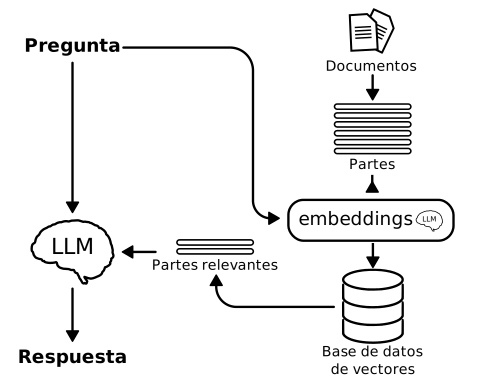
\includegraphics[width = 0.5\textwidth]{\DirFigCdos/simple_rag}
    \caption{Diagrama de funcionamiento de un esquema de RAG simple.}
    \label{fig:rag}
\end{figure}

\subsection{Indexado}

En su forma más simple, una base de conocimiento para RAG parte de la recolección
de documentos relacionados con las preguntas posteriores. Una de las ventajas
es que no hay limitante en la cantidad o tamaño, aunque si deben estar en
formato de texto. Estos documentos se separan en framentos, comunmente
llamados \textit{chunks}, el objetivo es obtener fragmentos pequeños pero
que contengan suficiente información. Posteriormente se calcula la
representación vectoriale (\textit{embedding}) de cada framento, para finalmente
almacenar cada fragmento con su respectivo \textit{embedding} en una base
de datos.

\subsection{Recuperación}

Dada una solicitud hecha al LLM, la recuperación consiste
en buscar información relevante, usualmente en forma de fragmentos de
documentos, en una base de datos previamente construida. La forma de
determinar si un fragmento es relevante o no para la pregunta se mide la
distancia entre la solicitud y el fragmento.

Una de las formas más comunes de medir esta distancia es empleando la
distancia coseno, en su forma de similitud coseno, como se muestra en la
ecuación \ref{eq:cos_similarity}

\begin{equation}\label{eq:cos_similarity}
    d = 1.0 - \frac{\sum{(A_i \times B_i)}}{\sqrt{\sum{(A_i^2)}}\sqrt{\sum{(B_i^2)}}}
\end{equation}

Otra de las métricas comunes es la distancia empleando el producto interno,
como se muestra en la ecuación \ref{eq:inner_product}.

\begin{equation}\label{eq:inner_product}
    d = 1.0 - \sum{(A_i \times B_i)}
\end{equation}

\subsection{Generación}

En esta etapa, tanto la solicitud como los documentos seleccionados son
sintetizados en una instrucción coherente que se le proporciona al modelo.
Usualmente esta instrucción incluye: Indicación de responder la pregunta
solamente con los fragmentos proporcionados, los fragmentos de texto y la
pregunta.

\section{Reentrenamiento de los modelos}

Tanto los LLMs comerciales como los de código abierto pasan por una serie de
pasos de entrenamiento y ajuste para funcionar adecuadamente en los
diferentes dominios para los que son preparados, de esta forma pueden ser
utilizados directamente sin modificaciones, sin embargo, en ocasiones es
posible mejorar su rendimiento en tareas específicas aplicando diferentes
técnicas de ajuste.

\subsection{Ingeniería de instrucciones (\textit{prompts})}

Cuando un modelo está entrenado para seguir instrucciones, es posible modificar
su comportamiento dando instrucciones adicionales que le sirvan como guía
al momento de dar la respuesta, a esto se le conoce como ingeniería de prompts.

Con esta técnica se puede instruir al modelo a realizar una serie de pasos
antes de dar la respuesta, modificar el tono, longitud o intención de la
respuesta, además de proporcionar información sobre la situación en que
se debe desempeñar.

\subsection{Ajuste fino supervisado}

Consiste en tomar un dataset que contenga ejemplos del comportamiento que
se desea que aprenda el modelo, en este proceso suelen usarse
ejemplos con pares intrucción-respuesta, donde la respuesta tiene
las características que se desea que el modelo aprenda. En este proceso
solo la salida del modelo es modificada, mientras todo lo demás permanece
igual, lo cual permite reducir la cantidad de recursos necesarios.

\subsection{Aprendizaje por refuerzo}

El aprendizaje profundo consiste en entrenar al modelo para tomar decisiones
que maximicen una recompenza. En el caso de los modelos de lenguaje, uno
de los enfoques más utilizados es el aprendizaje por refuerzo con
retroalimentación humana (RLHF, Reinforcement Learning from Human Feedback),
el cual utiliza retroalimentación humana para optimizar modelos.

Esta técnica de ajuste es particularmente útil porque es posible hacer que
el modelo adquiera comportamientos que no son fáciles de modelar matemáticamente,
sin embargo, tiene la desventaja de que requiere intervención humana y es por
ello más lento.

\section{Documentos normativos}

Se entiende como documentos normativos a aquellos que contienen reglas o
normas que rigen la operación de una organización o un organismo dentro de la
misma, también pueden ser reglamentos de eventos o actividades específicas.

En la actualidad, la mayoría de los documentos normativos de cualquier
organización se encuentran digitalizados en formato PDF y, en ocasiones, disponibles
en servidores web para que los miembros de las organizaciones puedan consultarlos
en cualquier momento.

En el caso de la normativa de la Universidad de Guanajuato, y de muchas otras
normativas, la estructura de los documentos se divide principalmente en:
Título, Sección, Capítulo y Artículos. Este trabajo pretende aprovechar esta
estructura predefinida para referenciar las repuestas del sistema.

\subsection{Formato PDF}

El formato PDF (Portable Document Format) es un formato cuyo objetvio es
ofrecer una forma sencilla y segura de presentar e intercambiar documentos con
independencia del software, el hardware o el sistema operativo que utilice quien
los consulte, con este fin, se encuentra estandarizado por la
ISO (Organización Internacional de Normalización) bajo la ISO 32000-1:2008
(PDF 1.7) y más recientemente la ISO 32000-2:2020 (PDF 2.0) [cita ISO].

Sin embargo, el formato PDF fue pensado como una herramienta para presentar
documentos en una forma entendible por humanos, es decir, no está
diseñado para que una máquina interprete su contenido de forma fácil, sino
para que un humano lo haga.

\subsection{Herramientas de extracción de texto}

Los LLMs operan con entradas de texto, si los documentos a ser empleados
se encuentran en formato PDF es necesario extraer la información textual que
contienen, para ello existen diferentes herramientas, sin embargo, el
resultado suele presentar errores errores o limitaciones propias del formato
PDF, como son la presencia de encabezados y pies de página entre el contenido
del documento, la falta de información sobre títulos, subtítulos o divisiones
de secciones, la dificultad para leer tablas, entre otras.

En el Apéndice A se encuentra una lista de las herramientas más comunes y
sus limitantes, la cual se emplea para seleccionar la herramienta más apta.

Dependiendo de la herramienta a emplear se debe hacer un procesamiento del
archivo PDF para eliminar los defectos e información que no sea relevante,
este proceso se presenta como parte de la metodología del proyecto.

\section{Trabajos relacionados}

En un esfuerzo por implementar una arquitectura robusta para hacer QA
desde diferentes fuentes de inforamción, Christmann \& Weikum
\cite{christmann_rag-based_2024} presentaron el sistema QUASAR, el cual emplea una
arquitectura basada en RAG para responder preguntas desde texto sin estructura,
tablas y grafos de conocimiento. Este sistema procesa las preguntas en
diferentes etapas, que denomina: Entendimiento de la pregunta, recuperación
de evidencia y reclasificación y filtrado. Con esta metología alcanzó
resultados superiores a modelos grandes como GPT-4 y Llama 3 en los benchmarks
CompMix \cite{christmann_compmix_2024} y TimeQuestions \cite{jia_complex_2021}
con un modelo Llama 3.1-8B-instruct
\footnote{https://huggingface.co/meta-llama/Llama-3.1-8B-Instruct}.

Al ser sistemas basados en RAG, nuestro sistema comparte elementos comunes
con el sistema QUASAR, sin embargo, nuestro trabajo pretende aprovechar
la estructura semi-estandarizada de los documentos normativos para realizar
una separación más eficiente de los documentos, además, la restricción
del dominio de las preguntas a documentos específicos, permite construir
una base de datos de conocimiento más sencilla, tanto en tamaño como en
pasos de procesamiento, lo que generaría un sistema más rápido y compacto.

Uno de los problemas principales del RAG es la recuperación de fragmentos
relevantes de los documentos, trabajos como el de Shao et al. \cite{shao_enhancing_2023}
se centran en proponer mejores técnias en la identificación de
documentos relevantes en cuerpos muy grandes de datos aplicando una
sinergia entre el recuperador y el generador para mejorar la respuesta
de forma iterativa. Otra forma de atender este problema lo presenta
Shi et al. con su framework RePlug \cite{shi_replug_2024}
el cual consiste en tratar al modelo de lenguaje que responde la pregunta
como un modelo de caja negra, mientras que el recuperador de información
es el que se entrena y ajusta, de esta forma mejora la capacidad de
QA del modelo sin tener que reentrenarlo. Es por esas consideraciones
que el sistema que se propone en este proyecto considera una etapa de ajuste
fino para el modelo que obtiene los \textit{embeddings} de los documentos,
el cual funciona como recuperador.

Por último, existen herramientas comerciales y de código abierto con la
capacidad de ejecutar metodologías RAG para responder a preguntas de documentos,
siendo el más usado ChatGPT
\footnote{https://help.openai.com/en/articles/8868588-retrieval-augmented-generation-rag-and-semantic-search-for-gpts},
el cual permite generar chats personalizados
y proporcionar una serie de documentos como contexto, al habilitar la opción
de "Recuperación de conocimiento", la herramienta aplica RAG y responde
las preguntas correspondientes. Otra heramienta con características
similares es LMStudio
\footnote{https://lmstudio.ai/docs/app/basics/rag},
la cual es de código abierto y permite el uso de
diferentes modelos, así como su ejecución en entornos locales.

A pesar de las bondades de las herramientas existentes, éstas
ponen sobre el usuario la responsabilidad de encontrar los documentos
requeridos y proporcionarlos a la herramienta, además tienen un límite de
documentos a subir y cuando el chat crece mucho, se debe reiniciar y volver
a repetir el proceso. Otras desventajas son que las respuestas no pueden ser
correctamente referenciadas a su artículo específico o que pueden incluir texto
indeseado como encabezados, pies de página o malas interpretaciones de la
secuencia del texto.

Son estos problemas los que se busca resolver en este proyecto al proporcionar
una herramienta que esté lista para usarse, sea de código abierto, proporcione
respuestas referenciadas correctamente y permita un nivel de personalización
completo para la institución.

%\chapter{Metodología}

En este capítulo se presentan las herramientas y pasos a seguir para la implementación
del sistema. Se comienza dando un panorama general del sistema, para posteriormente
describir la fuente de información normativa, así como los pasos de
implementación del asistente, que se divide en cuatro componentes:
Extactor de información, modelador de lenguaje, API de
comunicación y aplicación web. Posteriormente, se presenta la metodología
de evaluación de los modelos que componen el sistema, para finalmente
explicar el método de reentrenamiento del modelo de \textit{embeddings}.

\section{Panorama general}

El desarrollo del asistente requiere el uso de múltiples lenguajes de programación,
\textit{frameworks} y librerías. Se emplean las librerías \textit{transformers}
y \textit{llama\_cpp} de \textit{Python} para ejecutar los modelos LLM,
así como \textit{FastAPI} para programar la API de comunicación. Además,
se usa \textit{Javascript} (\textit{NextJS} y \textit{React}) para desarrollar la
aplicación web.

En la Figura \ref{fig:esquema_general} se muestran los cuatro módulos que
componen el sistema, en donde el procesamiento de la información comienza previo
a la interacción de un usuario, en el extractor de información.
El extractor obtiene el contenido de los documentos y lo fragmenta,
transforma los fragmentos en \textit{embeddings} y, finalmente, almacena
los \textit{embeddings} en una base de datos.
Una vez lista la base de datos, el usuario accede a la aplicación web,
desde donde realiza una pregunta que se envía al modelador de lenguaje a través
de la API de comunicación. Cuando el modelador de lenguaje recibe la pregunta,
el controlador busca en la base de datos los fragmentos de información relacionados
con la pregunta y se los proporciona al LLM como contexto, para que genere la respuesta. Una vez
obtenida la respuesta, el controlador la envía de vuelta a través de la API para que
el usuario pueda visualizarla en la aplicación web.

\begin{figure}[]
    \centering
    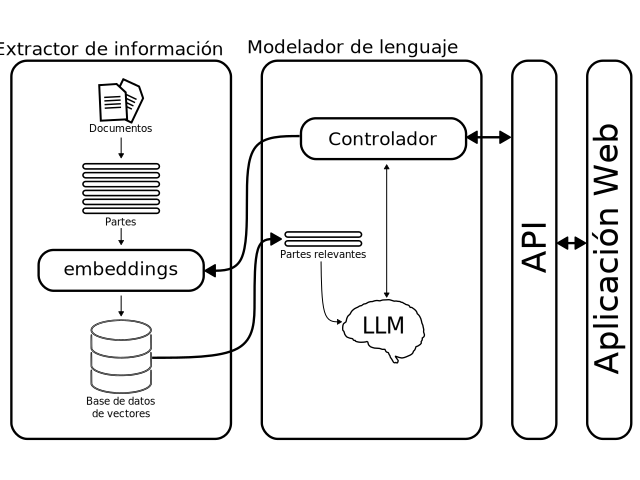
\includegraphics[width = 0.8\textwidth]{\DirFigCtres/esquema_general}
    \caption{Diagrama de componentes que conforman el sistema.}
    \label{fig:esquema_general}
\end{figure}

Para el desarrollo y puesta en producción de este proyecto se cuenta con
una estación de trabajo \textit{Dell Precision 7920 Tower} con un procesador
\textit{Intel\textregistered Xeon\textregistered Silver 4214R @2.40Ghz}, 256 GB de RAM
DDR5, un disco SSD \textit{Samsung PM881 SATA 52 GB}, un disco SSD
\textit{ADATA SU800 1TB}, dos GPUs \textit{Nvidia Quadro P620} de 2 GB de VRAM,
una GPU \textit{Nvidia RTX A4000} de 16 BG de VRAM y con sistema operativo
Windows 11. Además, se obtuvo acceso durante cuatro meses al centro de
supercómputo del CIMAT, a través de la convocatoria
\textit{Supercómputo como motor de colaboraciones académia-industria 2025},
para usar un nodo de cómputo GPU con dos tarjetas \textit{Nvidia TITAN RTX}
de 24 GB de VRAM cada una, con Ubuntu 22.04.5. Adicionalmente, se cuenta con una laptop de desarrollo
\textit{Dell G3 15} con una GPU \textit{Nvidia GTX 1050Ti} de 4 GB de VRAM y
con Ubuntu 24.04.02. Por último, para la puesta en producción del sistema
se tiene una licencia de estudiante de Azure con \$100 USD de crédito.

\section{Fuente de información}

El sistema está diseñado para responder preguntas de la normativa de la
Universidad de Guanajuato, esta normativa se encuentra disponible en la página
oficial de la universidad\footnote{https://www.ugto.mx/gacetauniversitaria/normatividad/normatividad-vigente}
en forma de 22 documentos PDF individuales. Cada documento tiene un número
diferente de páginas, las cuales suman 511, representan 6.8 MB de información y,
convertidas a texto, 168,011 palabras. Para alimentar la base de datos,
los documentos son descargados manualmente y almacenados en un directorio,
donde se utiliza el nombre del archivo como identificador. En la Tabla
\ref{tab:documentos} se muestra un resumen de los documentos que conforman
la normativa, así como el número de artículos que contiene cada uno.

\begin{table}[!ht]
    \centering
    \begin{tabular}{|c|l|r|r|}
        \hline
        N  & Nombre del documento                   & Artículos & Transitorios \\ \hline
        1  & Código de Conducta e Integridad ...    & 13        & 2            \\ \hline
        2  & Código de Ética de las Personas ...    & 7         & 1            \\ \hline
        3  & Código de Ética de la Universidad ...  & NA        & 1            \\ \hline
        4  & Estatuto Orgánico de la ...            & 91        & 8            \\ \hline
        5  & Ley Orgánica de la Universidad ...     & 75        & 8            \\ \hline
        6  & Reglamento Académico de la ...         & 101       & 11           \\ \hline
        7  & Reglamento de Becas, Apoyos y ...      & 39        & 5            \\ \hline
        8  & Reglamento de Bienes del ...           & 28        & 6            \\ \hline
        9  & Reglamento de Distinciones ...         & 21        & 4            \\ \hline
        10 & Reglamento de la Defensoría de ...     & 42        & 8            \\ \hline
        11 & Reglamento de la Junta Directiva ...   & 38        & 0            \\ \hline
        12 & Reglamento del Personal Académico ...  & 98        & 7            \\ \hline
        13 & Reglamento del Programa de ...         & 38        & 4            \\ \hline
        14 & Reglamento de Mecanismos Alternos ...  & 37        & 5            \\ \hline
        15 & Reglamento de Quienes Integran ...     & 31        & 9            \\ \hline
        16 & Reglamento de Responsabilidades ...    & 53        & 7            \\ \hline
        17 & Reglamento de Transparencia y ...      & 52        & 3            \\ \hline
        18 & Reglamento Editorial de la ...         & 35        & 1            \\ \hline
        19 & Reglamento Interno del Patronato ...   & 17        & 2            \\ \hline
        20 & Reglamento para la Incorporación ...   & 49        & 5            \\ \hline
        21 & Reglamento de Responsabilidades ...    & 30        & 11           \\ \hline
        22 & Modelo Educativo de la Universidad ... & NA        & NA           \\ \hline
    \end{tabular}
    \caption{Resumen de documentos normativos de la Universidad de Guanajuato}
    \label{tab:documentos}
\end{table}

\section{Extractor de información}

La labor del módulo de extracción de información comienza con un
archivo en formato PDF y termina con la creación de una base de datos de
\textit{embeddings} de los fragmentos del documento. En la Figura
\ref{fig:esquema_extractor} se observa la secuencia de procesamiento para un
archivo y la salida de cada una de las etapas.

\begin{figure}
    \centering
    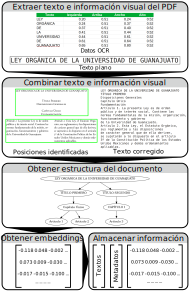
\includegraphics[width = 0.8\textwidth]{\DirFigCtres/esquema_extractor}
    \caption{Diagrama de extracción de información de un archivo PDF.}
    \label{fig:esquema_extractor}
\end{figure}

\subsection{Extraer texto e información visual del PDF}

Cada documento PDF debe convertirse a texto para su procesamiento,
conservando la información del formato y ubicación de los bloques de texto con el fin de
poder extraer la estructura de títulos y secciones del documento. Por lo anteror,
se extraen dos tipos de datos del archivo: texto plano e información visual
relacionada con el formato.

Para seleccionar las herramientas de extracción de texto plano se hizo un
análisis de aquellas que fueran de código abierto, considerando sus
deficiencias en la extracción de texto (ver Apéndice A). Se seleccionó
\textit{PyPDF}, porque es la herramienta más usada para esta tarea con Python, y
\textit{PdfPlumber}, porque su extracción de texto es la más limpia y provee mecanismos
para extraer la información visual.

El primer paso del procesamiento es extraer el texto plano con \textit{PyPDF} o \textit{PdfPlumber}. En el caso de PyPDF
no se puede obtiener información visual que ayude a identificar los títulos, secciones
y encabezados, además en ocasiones modifica el orden del texto. Para solucionar
estos problemas se utiliza la herramienta \textit{Tesseract}, la cual es un software de
reconocimiento óptico de caracteres (OCR, Optical Character Recognition)
que permite obtener la posición, ancho, alto y texto de
cada palabra dentro del documento (Figura \ref{fig:visual_info}). Para emplear Tesseract, primero se convierte el
documento a imágenes con una densidad de pixeles de 1000 DPI con \textit{PDF2Image}, para
posteriormente procesar cada imagen con la librería \textit{PyTesseract}.
Por otra parte, cuando se usa \textit{PdfPlumber}, el texto va acompañado de la información
visual necesaria, por lo que no es necesario emplear otras herramientas.

\begin{figure}
    \centering
    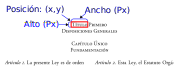
\includegraphics[width = 0.8\textwidth]{\DirFigCtres/visual_info}
    \caption{Ejemplo de información visual obtenida por \textit{Tesseract} y
        \textit{Pdfplumber}.}
    \label{fig:visual_info}
\end{figure}


\textit{Tesseract} es una herramienta, desarrollada por \textit{Google}, que puede reconstruir
el texto del documento, así como detectar las líneas, párrafos y secciones,
sin embargo, con frecuencia comete errores en la detección del texto y el
ordenamiento. Para corregir estos errores se propone combinar el texto
plano obtenido con \textit{PyPDF}, con la información de posición y tamaño devuelta
por \textit{Tesseract}, de esta forma se obtiene el texto correcto asociado a su
ubicación y tamaño. Este proceso se describe en el diagrama de la Figura
\ref{fig:texto_y_ocr}.

\begin{figure}[]
    \centering
    \includegraphics[width = 0.8\textwidth]{\DirFigCtres/esquema_texto_y_ocr}
    \caption{Detalle extracción de texto y características de OCR.}
    \label{fig:texto_y_ocr}
\end{figure}

Para el caso de PdfPlumber, la librería devuelve las mismas características que
PyTesseract, sin embargo, comete también errores en la agrupación y el
ordenamiento del texto, por ello se requiere realizar los pasos de ``Crear
grupos para reconstruir el texto'' y ``Reconstruir texto'' del diagrama de la Figura
\ref{fig:texto_y_ocr}.

La tarea de agrupar el texto en secciones para reconstruirlo en el orden correcto
no es trivial, y es altamente dependiente del tipo de documento a procesar.
Este proceso se explica en los diagramas de las Figuras
\ref{fig:reconstruccion_texto_1} y \ref{fig:reconstruccion_texto_2}, y
funciona adecuadamente para documentos donde predomina el texto en una o dos
columnas con títulos centrados, pero podría fallar cuando la estructura del
documento difiera considerablemente.

\begin{figure}[]
    \centering
    \includegraphics[width = 0.8\textwidth]{\DirFigCtres/reconstruccion_texto_ocr_1}
    \caption{Detalle de reconstrucción de texto del documento (Pt. 1).}
    \label{fig:reconstruccion_texto_1}
\end{figure}

\begin{figure}[]
    \centering
    \includegraphics[width = 0.8\textwidth]{\DirFigCtres/reconstruccion_texto_ocr_2}
    \caption{Detalle de reconstrucción de texto del documento (Pt 2).}
    \label{fig:reconstruccion_texto_2}
\end{figure}

Una vez realizada la agrupación de los elementos de la página, es posible reconstruir
el texto respetando el orden normal de lectura, eliminando los errores de
posicionamiento de \textit{PyPDF} o \textit{PdfPlumber} según sea el caso.
Además, cuando se utiliza \textit{PyPDF}+\textit{Tesseract}, el texto contiene
errores de detección de texto que serán corregidos al combinar la información
visual del texto reconstruido, con el texto plano extraído con \textit{PyPDF}.

\subsection{Combinar texto e información visual}

Cuando se usa \textit{PdfPlumber}, este proceso no es necesario, pues la librería ya
devuelve el texto correcto asociado a su información visual de posición y tamaño,
sin embargo, cuando se usa \textit{PyPDF}+\textit{PyTesseract}, es necesario combinar estas dos
fuentes de información para obtener el texto y la información visual correctas.
El objetivo es tener la posición de cada palabra asociada con su texto correcto,
de esta forma se podrá distinguir entre diferentes elementos, como títulos,
párrafos, entre otros.

El proceso de combinación requiere las cadenas de texto extraídas por los dos métodos:
la cadena proporcionada por \textit{PyPDF} y la cadena reconstruida con la información
visual, como se muestra en la Figura \ref{fig:reconstruccion_texto_2}. Ambas cadenas se
separan por palabra y se pasan a la librería \textit{Difflib}, la cual aplica el algoritmo
Ratcliff-Obershelp, también conocido como Coincidencia de patrones Gestalt, para
comparar dos cadenas y encontrar sus diferencias.

Si se analizan los patrones de salida de la librería \textit{Difflib}, es posible
corregir las palabas detectadas con OCR utilizando las palabras extraídas directamente
del texto, los detalles de esta implementación se explican en la Figura
\ref{fig:esquema_combinacion_txt_ocr}.
En escencia, se considera la palabra obtenida con \textit{PyPDF} como la correcta,
se compara contra la palabra obtenida con \textit{Tesseract} y si es diferente se sobreescribe.
Al terminar el proceso se tiene un arreglo de datos donde se conoce la posición
y dimensiones de cada palabra, así como su texto correcto, además se cuenta con
datos adicionales de línea, columna, alineación o grupo que serán empleadas
para dividir las secciones del documento más adelante.


\begin{figure}[]
    \centering
    \includegraphics[width = 0.8\textwidth]{\DirFigCtres/combinacion_texto_ocr}
    \caption{Detalle de combinación de texto plano con información de OCR.}
    \label{fig:esquema_combinacion_txt_ocr}
\end{figure}

Las ventajas de usar \textit{PdfPlumber} sobre \textit{PyPDF}+\textit{PyTesseract}
son que \textit{PdfPlumber} es más rápido y
la identificación del texto es certera, pues proviene directamente del archivo,
sin embargo, no funciona si el PDF es un escaneo o si contiene texto en forma
de imagen. Por su parte, al generar el método de \textit{PyPDF}+\textit{PyTesseract}, se desarrollaron
elementos que fueron reutilizados al usar \textit{PdfPlumber}, como la resconstrucción de texto.
Además, si se confía plenamente en la predicción de \textit{PyTesseract}, se
puede dar soporte a documentos escaneados o con imágenes con texto.

\subsection{Obtener estructura del documento}

El objetivo de este paso es generar una estructua de datos en la que cada parte
del documento esté referenciada a su sección y subsecciones correspondientes,
por ejemplo, para la Ley Orgánica se desea conocer en qué título, capítulo y
artículo se encuentra un texto específico. Para crear dicha estructura, se optó por generar un árbol, donde cada nodo
corresponde a una sección del documento, además, las hojas y los nodos intermedios
almacenan el texto de cada artículo o sección según sea el caso. En la Figura
\ref{fig:fragmento_arbol} se muestra una porción del árbol correspondiente a
las primeras secciones de la Ley Orgánica.

\begin{figure}[]
    \centering
    \includegraphics[width = 0.8\textwidth]{\DirFigCtres/fragmento_arbol}
    \caption{Porción del árbol del documento ``Ley Orgánica de la Universidad de Guanajuato''.}
    \label{fig:fragmento_arbol}
\end{figure}

Para generar el árbol es necesario analizar el documento en varios pasos. Primero,
se divide el documento en bloques de texto que estén separados verticalmente,
es decir, que haya al menos una línea en blanco entre ellos.
Posteriormente se detectan los bloques que corresponden a títulos, estos típicamente
se encuentran centrados en la página o en la columna. Para encontrar las
secciones o subsecciones se consideran los títulos centrados en la página
y se les asigna un nivel.
Para asignar el nivel se debe conocer de antemano la estructura del documento
y generar expresiones regulares que ayuden a diferenciar un título, de un subtítulo,
y así sucesivamente. Para los documentos normativos de la Universidad
de Guanajuato la estructura es la siguiente:

\begin{itemize}
    \item \textbf{Nivel 1 - Encabezado general:} Son textos abiertos que no tienen palabras o
          estructura específica y se consideran dentro del primer nivel.
          \begin{itemize}
              \item Sin expresión regular
          \end{itemize}
    \item \textbf{Nivel 2 - Título:} Los documentos se dividen en títulos. Cada título comienza con
          la palabra \textit{Título}. También pueden ser numerales romanos.
          \begin{itemize}
              \item \string^(título\textbar[xiv]+\textbackslash.) .*
          \end{itemize}
    \item \textbf{Nivel 3 - Sección (Opcional):} Algunos documentos dividen los títulos en secciones.
          Cada sección comienza con la palabra \textit{Sección}. También pueden ser
          secciones numeradas.
          \begin{itemize}
              \item \string^([0-9]+\.[0-9]|sección) .*
          \end{itemize}
    \item \textbf{Nivel 4 - Capítulo:} Los títulos o secciones se dividen en capítulos y cada capítulo comienza
          con la palabra \textit{Capítulo}
          \begin{itemize}
              \item \string^capítulo .*
          \end{itemize}
\end{itemize}

Además, se debe tener en cuenta que hay divisiones del documento
que no se encuentran centrados, sino que están contenidos en el grueso del
texto, como lo son los Artículos. Para identificar estas separaciones en el
contenido, también se crean expresiones regulares que se verifican contra el
inicio de cada bloque mientras se va construyendo el árbol.

\begin{enumerate}
    \item \textbf{Artículo:} Los capítulos tienen uno o más artículos.
          \begin{itemize}
              \item  \string^artículo ([0-9]+\textbar[a-zé]+(ro\textbar do\textbar ro\textbar to\textbar mo\textbar vo\textbar no\textbar único)\\
                    (bis\textbar ter\textbar quáter\textbar quinquies)?\textbackslash.
          \end{itemize}
\end{enumerate}

Una vez identificados los títulos y teniendo la forma para encontrar las
divisiones dentro del contenido, se recorre el documento. Recorrer
el documento es el equivalente a recorrer el árbol por profundidad, por lo
que se va creando el árbol de la misma forma, es decir, cuando se encuentra
un título se crea un nuevo nodo en el nivel correspondiente, siempre teniendo
la referencia de cual será su padre, cuando se llega al nivel más bajo se
guarda el contenido de texto en el nodo correspondiente.
El proceso completo se presenta en la Figura
\ref{fig:crear_arbol}.

\begin{figure}[]
    \centering
    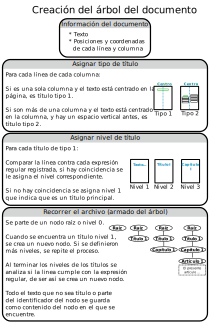
\includegraphics[width = 0.78\textwidth]{\DirFigCtres/crear_arbol}
    \caption{Proceso de creación del árbol de secciones de un documento.}
    \label{fig:crear_arbol}
\end{figure}

\subsection{Obtener \textit{embeddings}}

Para el cálculo de \textit{embeddings} se emplean modelos LLM de extracción de
\textit{embeddings}. El sistema propuesto permite el uso y evaluación de
varios modelos, los cuales serán: MiniLM (33M de parámetros)
\cite{wang_minilm_2020}, MPNET \cite{hagen_mpnet_2020} (110M de parámetros)
y Qwen 3 \cite{zhang_qwen3_2025} (600M, 4B y 8B de parámetros). Estos modelos
se encuentran disponibles en HuggingFace y se pueden
usar con las librearías \textit{SentenceTransformers} o \textit{Transformers}.

Los modelos MiniLM y MPNET fueron seleccionados por su tamaño reducido,
ya que pueden ejecutarse en CPU de forma eficiente. Los
modelos Qwen se seleccionaron ya que ocupan los primeros puestos en el
MTEB Ladderboard de HuggingFace\footnote{https://huggingface.co/spaces/mteb/leaderboard},
que clasifica modelos de extracción de \textit{embeddings} en diferentes idiomas
y con múltiples métricas. Además, con el objetivo de reducir el uso de memoria,
también se evalúan los modelos
cuantizados de Qwen 3: f16 (16 bits), Q8\_0 (8 bits), Q6\_K (6 bits), Q5\_K\_M (5 bits)
y Q4\_K\_M (4 bits). Estos modelos cuantizados se emplean con la librería \textit{llama\_cpp},
la cual es una implementación de la arquitectura \textit{Llama} de Meta en
C/C++ para hacer inferencia de forma eficiente. Un resumen de las características
de los modelos de extracción de \textit{embeddings} se encuentra en la Tabla \ref{tab:embed_models}.

\begin{table}[!ht]
    \centering
    \begin{tabularx}{0.8\textwidth}{|l|X|r|X|}
        \hline
        Modelo                     & Tipo de dato & Memoria  & Tamaño Embed. \\ \hline
        Qwen3-Embedding-0.6B       & BF16         & 3.65 GB  & 1024          \\ \hline
        Qwen3-Embedding-4B         & BF16         & 15.31 GB & 2560          \\ \hline
        Qwen3-Embedding-8B         & BF16         & 28.5 GB  & 4096          \\ \hline
        Qwen3-Embedding-0.6B-GGUF  & Q8\_0        & 2.51 GB  & 1024          \\ \hline
        Qwen3-Embedding-0.6B-GGUF  & F16          & 3.03 GB  & 1024          \\ \hline
        Qwen3-Embedding-4B-GGUF    & Q4\_K\_M     & 5.01 GB  & 2560          \\ \hline
        Qwen3-Embedding-4B-GGUF    & F16          & 10.18 GB & 2560          \\ \hline
        Qwen3-Embedding-8B-GGUF    & Q4\_K\_M     & 7.05 GB  & 4096          \\ \hline
        Qwen3-Embedding-8B-GGUF    & F16          & 16.82 GB & 4096          \\ \hline
        all-MiniLM-L6-v2           & I64/F32      & 144 MB   & 384           \\ \hline
        multi-qa-mpnet-base-dot-v1 & I64/F32      & 478 MB   & 768           \\ \hline
    \end{tabularx}
    \caption{Resumen de modelos de extracción de \textit{embeddings}}
    \label{tab:embed_models}
\end{table}

El proceso para convertir la información del documento a \textit{embeddings} consiste
en recorrer el árbol en profundidad, y en cada nodo hacer lo siguiente:

\begin{enumerate}
    \item Tomar el contenido textual del nodo, separarlo por párrafos y
          agrupar los párrafos en fragmentos de aproximadamente C caracteres.
          Cada fragmento será un registro independiente.
    \item Utilizar \textit{SentenceTransformers}/\textit{Transformers}/\textit{Llama\_cpp}
          para calcular el \textit{embedding} de cada fragmento y guardarlo como un vector de números.
    \item Obtener la ruta del nodo dentro del árbol. Ej: Ley Orgánica $\rightarrow$
          Título Primero $\rightarrow$ Capítulo segundo $\rightarrow$ Artículo 30.
    \item Guardar la ruta y el nombre del nodo como metadatos, así como el nombre
          del documento y cualquier información relevante.
\end{enumerate}

Al final, por cada fragmento se tendrá la siguiente información:

\begin{itemize}
    \item Texto del fragmento.
    \item \textit{Embedding} como vector de N valores numéricos.
    \item Metadatos:
          \begin{itemize}
              \item Nombre del documento.
              \item Ruta en el árbol.
              \item Nombre del nodo.
              \item Número de fragmento dentro del nodo.
              \item Nombre del nodo padre
          \end{itemize}
\end{itemize}

\subsection{Almacenar información}

Los \textit{embeddings} pueden almacenarse de varias formas en el disco siendo, las más
convenientes el formato CSV y las bases de datos con soporte para vectores.
El formato CSV tiene la ventaja de ser portable y fácil de leer, basta con
convertir los metadatos a formato JSON, para que puedan ser almacenados
como texto, mientras que el vector de \textit{embedding} se puede
expandir y crear una columna para cada valor. En la Figura \ref{fig:ejemplo_csv}
se muestra un ejemplo de la información almacenada como archivo CSV.
Este método funciona bien para hacer la evaluación y análisis de los modelos,
sin embargo, no es apto para entornos productivos, ya que no se tienen
optimizados para la búsqueda en los vectores de datos.

\begin{figure}[]
    \centering
    \includegraphics[width = 0.8\textwidth]{\DirFigCtres/ejemplo_csv}
    \caption{Ejemplo almacenamiento de metadatos y \textit{embeddings} en formato csv.}
    \label{fig:ejemplo_csv}
\end{figure}

Otra forma de almacenar los \textit{embeddings} es empleando una base de datos que
soporte vectores. El mayor beneficio de estas herramientas es que
permiten almacenar los datos de forma óptima, ya que la información
se puede agrupar en tablas, se puede agregar información adicional y
cuentan con funciones optimizadas de búsqueda por similitud de vectores.
Algunos ejemplos de estas bases de datos vectoriales son: Chroma, Marco o
PostgreSQL.

Este proyecto emplea ChromaDB, la cual funciona con SQLite y está diseñada para funcionar en
entornos productivos, y permite el uso de otras librerías para calcular
los \textit{embeddings}, como \textit{SentenceTransformers} y
\textit{llama\_cpp} u otro método personalizado, además, permite el
uso de diferentes parámetros de búsqueda por similitud semántica
como son la distancia coseno y el producto interno, los cuales también se
encuentran optimizados. En la Figura \ref{fig:ejemplo_chromadb} se muestra
un ejemplo de datos almacenados en ChromaDB.

\begin{figure}[]
    \centering
    \includegraphics[width = 0.8\textwidth]{\DirFigCtres/ejemplo_chromadb}
    \caption{Ejemplo de cómo se almacenan metadatos en Chroma DB. Los vectores
        se almacenan de forma óptima en un archivo separado.}
    \label{fig:ejemplo_chromadb}
\end{figure}

\section{Modelador de lenguaje}

El modelador de lenguaje tiene dos funciones fundamentales: manejar la
interacción con la base de datos de vectores y hacer uso del
LLM de inferencia principal, en términos de RAG, se encarga de la
recuperación y la generación. El proceso general que ejecuta el modelador
de lenguaje se presenta en el diagrama de la Figura
\ref{fig:esquema_modelador} y se explica en las siguientes subsecciones.

\begin{figure}
    \centering
    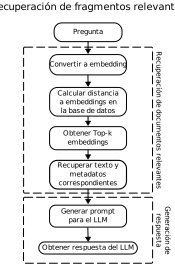
\includegraphics[width = 0.75\textwidth]{\DirFigCtres/esquema_recuperacion}
    \caption{Pasos seguidos por el modelador de lenguaje para procesar una pregunta.}
    \label{fig:esquema_modelador}
\end{figure}

\subsection{Recuperación de fragmentos relacionados}

Dada una pregunta, el modelador la convierte a \textit{embedding}
empleando el mismo modelo usado en la base de datos de vectores. Este \textit{embedding}
se le proporciona a ChromaDB para que realice la búsqueda semántica, el parámetro
de búsqueda puede ser por producto interno o por similitud coseno, dependiendo
del modelo de \textit{embedding}. Para hacer una búsqueda eficiente,
ChromaDB emplea un índice llamado HNSW (Hierarchical Navigable Small World),
esto le permite encontrar los fragmentos con mayor similitud a la pregunta
sin tener que comparar con toda la base de datos.

Con ChromaDB se obtiene el top \textit{k} de \textit{embeddings} similares
al \textit{embedding} de la pregunta, por defecto \textit{k} se establece
en 5. De estos \textit{k} \textit{embeddings} se obtiene su texto original,
su posición dentro del árbol del documento, el documento al que pertenece
y los demás metadatos del fragmento.

\subsection{Generación de respuesta}

Para la generación de la respuesta, se emplea un modelo multidominio de código
abierto. Para seleccionar el modelo óptimo para el sistema se seleccionaron
distintos modelos cuya restricción principal es que pudieran ejecutarse en el
hardware del sistema, es decir, que funcionen correctamente con 16 GB de VRAM.
Se evaluarán los modelos Qwen 3 \cite{zhang_qwen3_2025} (600M y 8B de parámetros)
en sus versiones completas y cuantizadas, Llama 3.1 (8B de parámetros)
y el modelo GPT-OSS (20B de parámetros) en su versión cuantizada.

\begin{table}[!ht]
    \centering
    \begin{tabular}{|l|l|l|l|l|l|}
        \hline
        Modelo                & Tipo de dato & Memoria  & Herramienta  \\ \hline
        Qwen3-0.6B            & BF16         & 1.74 GB  & Transformers \\ \hline
        Qwen3-8B              & BF16         & 15.59 GB & Transformers \\ \hline
        Qwen3-8B-Q4\_K\_M     & Q4\_K\_M     & 7.07 GB  & Llama\_cpp   \\ \hline
        gpt-oss-20b-MXFP4     & MXFP4        & 13.76 GB & Llama\_cpp   \\ \hline
        Llama-3.1-8B-Instruct & BF16         & 15.27 GB & Transformers \\ \hline
    \end{tabular}
    \caption{Resumen de modelos de generación de respuesta.}
    \label{tab:llm_models}
\end{table}

Para la evaluación inicial, a todos los modelos se les configura una instrucción
de sistema simple que le indica que su propósito es ser un asistente, esto
con el objetivo de evaluarlos en su forma básica.

\begin{verbatim}
    Eres un asistente que ayuda a responder preguntas.
\end{verbatim}

En una segunda evaluación, se comparan únicamente los mejores modelos de la primera etapa,
pero esta vez con una instrucción de sistema más compleja, donde se incluyen instrucciones
de cómo procesar las preguntas, el tono en que debe contestar, entre otros elementos.
Esta instrucción es más cercana a la que se usará en la aplicación final y
se puede consultar en el Apéndice B.

Teniendo la pregunta y los fragmentos relacionados con la misma, con sus metadatos,
se transmite la información al LLM a través de una instrucción con la plantilla
mostrada a continuación, que contiene la pregunta, y los fragmentos
relacionados en formato JSON con toda su información.

\begin{verbatim}
<pregunta>
{pregunta}
</pregunta>

<contexto>
{documentos_en_JSON}
</contexto>
\end{verbatim}

Un ejemplo de una instrucción completa se muestra a continuación:

\begin{verbatim}
<pregunta>
¿Qué contiene la Ley Orgánica de la Universidad de Guanajuato?
</pregunta>

<contexto>
[
    {
        "documento": "ley-organica-de-la-universidad
                      -de-guanajuato",
        "nombre": "Artículo 1",
        "contenido": "La presente Ley es de orden
                      público y de interés social. Contiene
                      las normas fundamentales de la misión,
                      organización, funcionamiento y
                      gobierno de la Universidad de
                      Guanajuato."
    },
    {...}
]
</contexto>
\end{verbatim}

La instrucción generada se le proporciona al modelo junto con
el historial anterior del chat para obtener la
respuesta. Por lo general, la respuesta a la pregunta
del usuario se encuentra únicamente en uno o dos fragmentos, pero al modelo
se le proporcionan k fragmentos como contexto. Para lograr que en
la aplicación web se le muestre al usuario únicamente los fragmentos
de los que se extrajo la respuesta, se aprovecha la capacidad pre-entrenada
del modelo de referenciar su respuesta, pero se mejora al agregar al comando del sistema una línea
adicional para indicar que debe referenciar los fragmentos como
una lista en formato JSON al final de la respuesta.
Se teoriza que al proporcionar al modelo los fragmentos de forma estructurada
en un JSON, se puede solicitar que haga referencia a campos específicos de los
mismos también en formato JSON, el cual es un formato que la aplicación
puede interpretar fácilmente.
El comando adicional de sistema se muestra a continuación y sólo se
agrega en el sistema final y no para las evaluaciones de los modelos.

\begin{verbatim}
Si la respuesta se encuentra en uno o varios artículos o
secciones específicas, cítalos al final de tu respuesta en
formato JSON de la siguiente manera:
<documents>[{"documento": [Nombre del Documento],
"nombre": [Artículo/Sección]}]</documents>.
Si el nombre del documento o artículo no está disponible en
el fragmento, omite la cita.
\end{verbatim}

Un ejemplo de una respuesta del modelo con esta instrucción se muestra
a continuación:

\begin{verbatim}
La Ley Orgánica de la Universidad de Guanajuato contiene
las normas fundamentales que establecen la misión, la
organización, el funcionamiento y el gobierno de la
Universidad, y se caracteriza por ser de orden público
y de interés social.

<documents>
[
    {
        "documento": "ley-organica-de-la-universidad
                      -de-guanajuato",
        "nombre": "Artículo 1",
    }
]
</documents>
\end{verbatim}


\section{API de comunicación}

La tarea de la API es conectar la aplicación web con el modelador de lenguaje.
La API funciona con peticiones HTTP de tipo POST y expone un solo endpoint
que recibe parámetros en formato JSON, además esta protegida con un API-KEY
que se debe enviar en el encabezado de cada petición. Un ejemplo de petición
se muestra en la Figura \ref{fig:parametros_api}. La estructura de una petición es la siguiente:

\begin{itemize}
    \item \textbf{model:} Identificador del modelo a emplear.
    \item \textbf{num\_related\_questions:} (Opcional) Número de preguntas previas a tomar
          en cuenta para buscar fragmentos relacionados a la pregunta actual. Por defecto 1.
    \item \textbf{messages:} Lista de mensajes.
          \begin{itemize}
              \item \textbf{role:} Rol del mensaje. ``system'', ``user'' o ``assistant''.
              \item \textbf{content:} Texto de la pregunta, respuesta o instrucción.
          \end{itemize}
\end{itemize}

\begin{figure}[]
    \centering
    \includegraphics[width = 0.8\textwidth]{\DirFigCtres/parametros_api}
    \caption{Ejemplo de petición a API.}
    \label{fig:parametros_api}
\end{figure}

La respuesta de la API también es en formato JSON y contiene el texto de la
respuesta, así como los fragmentos de los documentos que fueron tomados como contexto para
emitirla, como se muestra en la Figura \ref{fig:respuesta_api}. En estos
documentos, se incluyen los metadatos para poder desplegarlos en la aplicación
web. La estructura de la respuesta es la siguiente:

\begin{itemize}
    \item \textbf{iderror:} Identificador del error. 0 en caso de que no haya error.
    \item \textbf{msgerror:} Mensaje de error, en caso de haberlo.
    \item \textbf{choices:} Respuesta del modelo, como arreglo de respuestas, aunque
          solo sea una.
          \begin{itemize}
              \item \textbf{content:} Contenido de texto de la respuesta.
              \item \textbf{metadata:} Metadatos de los fragmentos de referencia.
                    \begin{itemize}
                        \item \textbf{title:} Título de la sección.
                        \item \textbf{path:} Ruta del fragmento en la estructura del documento.
                        \item \textbf{document\_name:} Nombre del documento de referencia.
                        \item \textbf{parent:} Nombre de la sección donde se encuentra el fragmento.
                    \end{itemize}
          \end{itemize}
\end{itemize}

\begin{figure}
    \centering
    \includegraphics[width = 0.8\textwidth]{\DirFigCtres/respuesta_api}
    \caption{Ejemplo de respuesta de API.}
    \label{fig:respuesta_api}
\end{figure}

\section{Aplicación web}

La aplicación web es la única forma de interacción de los usuarios con el
sistema, es por ello que debe contener todas las funcionalidades necesarias
que en este caso son: ingresar una pregunta, recibir una respuesta y
consultar los documentos que dan fundamento a dicha respuesta. Con este fin,
la aplicación web debe contar con una caja de texto para hacer la pregunta
y una lista de mensajes enviados y recibidos como un chat
convencional. Adicionalmente, se debe destinar un espacio para colocar los
fragmentos de los documentos relacionados con la pregunta, como se muestra en el
\textit{wireframe} de la Figura \ref{fig:wireframe_chat}.

\begin{figure}
    \centering
    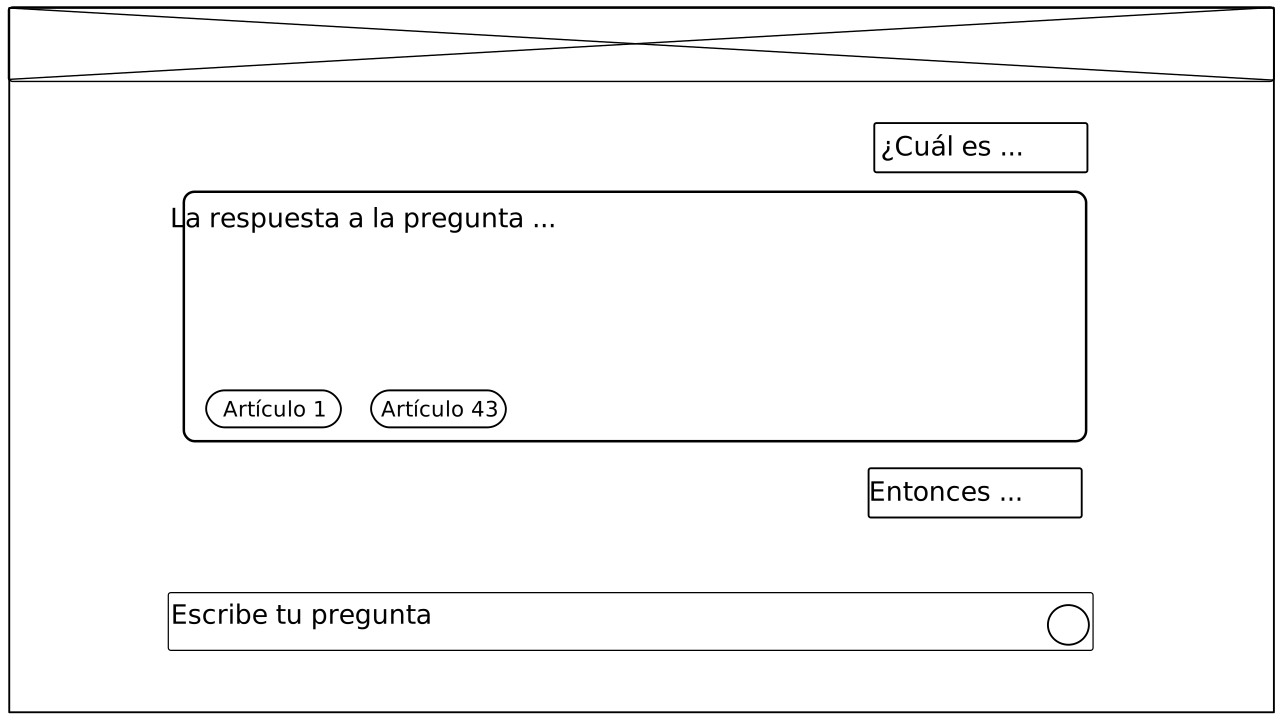
\includegraphics[width = 0.8\textwidth]{\DirFigCtres/wireframe_chat}
    \caption{Esqueleto del chat de la aplicación.}
    \label{fig:wireframe_chat}
\end{figure}

Con el fin facilitar el uso de la aplicación, no será obligatorio crear
una cuenta de usuario para hacer uso de la misma, sin embargo, se puede agregar
la funcionalidad como opcional, para que los usuarios registrados puedan
conservar el historial de conversaciones a largo plazo, así como acceder
desde distintos dispositivos. En caso de no crear una cuenta, los chats
solo estarán disponibles por 7 días, siempre y cuando el usuario no
elimine las cookies de su navegador. Adicional a esto, otras funcionalidades
se deben agregar como el visualizar el historial de chat o eliminar chats.
Para cubrir todas las funcionalidades se diseña la estructura de base de
datos de la Figura \ref{fig:chatug_db} para que sea implementada.

\begin{figure}
    \centering
    \includegraphics[width = 0.8\textwidth]{\DirFigCtres/chatug_db}
    \caption{Esquema de tablas de la base de datos de la aplicación.}
    \label{fig:chatug_db}
\end{figure}

\section{Evaluación de los modelos}

Para seleccionar los modelos de extracción de \textit{embeddings} y de
inferencia más aptos, se realiza una evaluación en varios pasos, donde de cada paso
se seleccionan los mejores modelos, hasta llegar a la mejor combinación
considerando rendimiento y recursos.

\subsection{Conjunto de datos de evaluación}

Es necesario generar un conjunto de datos de preguntas y respuestas
de los documentos normativos, con el fin de conocer el rendimiento
de los modelos en este dominio específico.
Tres personas fungen como los generadores de preguntas, a cada una se le
proporcionan 7 u 8 documentos, para completar el total de 21, se
excluye el documento denominado ``Modelo Educativo de la Universidad
de Guanajuato y su Modelo Académico'' pues no se encuentra divido en
artículos y dificultaría la referenciación de las respuestas. Se instruye a cada
participante para que genere de 1 a 4 preguntas por cada artículo de cada
documento, ignorando los textos introductorios. Cada pregunta debe
contener la siguiente información: pregunta, respuesta y contexto.
La pregunta debe redactarse de forma natural, mientras que la respuesta debe encontrarse
directamente en el artículo correspondiente del documento y debe ser copiada
directamente del mismo, por último, el contexto corresponde al nombre del
artículo de donde fue extraída la pregunta.

La base de datos se genera en formato CSV, por conveniencia de los
participantes, pero después se convierte a JSON y complementa con
otros campos pertinentes para que sea similar a la estructura del
conjunto de datos SQuAD \cite{rajpurkar_squad_2016}.
Posteriormente, el conjunto de datos se carga en
la plataforma HuggingFace como un conjunto de datos de QA por conveniencia.
Una entrada del conjunto de datos final contiene los siguientes elementos:

\begin{itemize}
    \item \textbf{id:} Identificador único de la pregunta. Es un MD5.
    \item \textbf{title:} Nombre del documento.
    \item \textbf{context:} Nombre del artículo donde se encuentra la respuesta.
    \item \textbf{context\_text:} Texto plano del artículo donde se encuentra la respuesta.
    \item \textbf{additional\_context:} En caso de que el artículo haga referencia a otro documento o artículo se incluye aquí.
    \item \textbf{question:} Texto de la pregunta.
    \item \textbf{anwers:}
          \begin{itemize}
              \item \textbf{text:} Arreglo con las cadenas de respuesta a la pregunta. Usualmente solo es una.
          \end{itemize}
\end{itemize}

\subsection{Evaluación del modelo de \textit{embedding}}

El objetivo de esta evaluación es conocer la calidad de los fragmentos
identificados como relacionados con cada pregunta.
Se emplearán tres métricas: \textit{precision@k}, \textit{recall@k} y
\textit{f1@k}. Cada una de estas métricas se definen con las ecuaciones
\ref{eq:precision}, \ref{eq:recall}, \ref{eq:f1} respectivamente. Para
aplicar estas fórmulas se necesita calcular la similitud entre la pregunta
y todos los fragmentos en la base de datos, compararlos y obtener
el top k con mayor similitud. Además, se debe considerar
como fragmento relevante a aquel que realmente contenga la respuesta a la
pregunta, lo cual se determina al comparar el nombre del nodo del
fragmento con el nombre del artículo marcado como contexto en el
conjunto de datos de evaluación.

\begin{equation}\label{eq:precision}
    \text{precision@k} = \frac{\text{N fragmentos relevantes en top k}}{k}
\end{equation}

\begin{equation}\label{eq:recall}
    \text{recall@k} = \frac{\text{N fragmentos relevantes en top k}}{\text{N fragmentos relevantes totales}}
\end{equation}

\begin{equation}\label{eq:f1}
    \text{f1@k} = \frac{2 \times \text{precision} \times \text{recall}}{\text{precision} + \text{recall}}
\end{equation}

El proceso de evaluación de los \textit{embeddings} se realiza siguiendo
los siguientes pasos:

\begin{enumerate}
    \item Para cada pregunta, se identifican los fragmentos relevantes. Es decir,
          los fragmentos de los artículos donde se encuentra la respuesta.
    \item Se calcula la similitud coseno entre la pregunta y cada fragmento de
          la base de datos de \textit{embeddings}, incluyendo todos los documentos.
    \item Se obtienen los k fragmentos con mayor similitud coseno.
    \item Se calculan las métricas de evaluación con los k fragmentos obtenidos.
    \item El proceso se repite con todas las preguntas del conjunto de datos y
          al final se obtienen las medias de cada métrica.
\end{enumerate}

\subsection{Evaluación del modelo de inferencia}

El objetivo de esta evaluación es conocer la similitud de la respuesta
candidata con la respuesta de referencia, y si la respuesta responde correctamente
la pregunta. Se emplearán tres métricas principales: puntuación ROUGE,
puntuación BERT y similitud coseno. ROUGE (Recall-Oriented Understudy for
Gisting Evaluation) es una métrica que evalúa la superposición entre una
oración candidata y otra de referencia, en específico, ROUGE-L emplea la
subsecuencia de texto en común más larga (LCS, Longest Common Subsequence)
para calcular la precisión, recall y la puntuación f1, como se muestra en
las fórmulas \ref{eq:precision_lcs}, \ref{eq:recall_lcs}, \ref{eq:f1_lcs}.

\begin{equation}\label{eq:precision_lcs}
    P_{LCS} = \frac{\text{N palabras en LCS}}{\text{N palabras en respuesta inferida}}
\end{equation}

\begin{equation}\label{eq:recall_lcs}
    R_{LCS} = \frac{\text{N palabas en LCS}}{\text{N palabras en referencia}}
\end{equation}

\begin{equation}\label{eq:f1_lcs}
    F1_{LCS} = \frac{2 \times P_{LCS} \times R_{LCS}}{P_{LCS} + R_{LCS}}
\end{equation}

La puntuación BERT consiste en tomar la respuesta candidata y la respuesta
de referencia, tokenizarla y obtener el \textit{embedding} de cada token con un modelo BERT.
Una vez obtenidos los \textit{embeddings}, se calcula la similitud coseno entre
cada token de la secuencia candidata $(\hat{x}_1, ..., \hat{x}_k)$ y cada
token de la referencia $(x_1, ..., x_m)$, para calcular la precisión y recall
empleando los tokens más similares, como se muestra en las ecuaciones
\ref{eq:precision_bert}, \ref{eq:recall_bert} y \ref{eq:f1_bert}.

\begin{equation}\label{eq:precision_bert}
    P_{BERT} = \frac{1}{|\hat{x}|}\sum_{\hat{x}_j \in \hat{x}}\max_{x_i \in x}x_i^T \hat{x}_j
\end{equation}

\begin{equation}\label{eq:recall_bert}
    R_{BERT} = \frac{1}{|x|}\sum_{x_i \in x}\max_{\hat{x}_j \in \hat{x}}x_i^T \hat{x}_j
\end{equation}

\begin{equation}\label{eq:f1_bert}
    F1_{BERT} = \frac{2 \times P_{BERT} \times R_{BERT}}{P_{BERT} + R_{BERT}}
\end{equation}

Por último, la similitud coseno se evalua calculando el \textit{embedding}
de la respuesta candidata y el de la respuesta referencia, para ello
se emplea un modelo simple de extracción de \textit{embeddings} como
el all-MiniLM-L6-v2 y se obtiene la similitud coseno entre ambos vectores.

\section{Reentrenamiento del modelo de \textit{embeddings}}

En este proyecto se emplea la forma más directa de reentrenamiento o ajuste
fino, que es el reentrenamiento completo del modelo sobre un conjunto
de datos especializados. El conjunto de datos será el descrito anteriormente
para la evaluación de los modelos, haciendo una división aleatoria de 80\%
de muestras para el entrenamiento y un 20\% para la evaluación. Esta
separación se hace a nivel archivo, por lo que se garantiza que exista al menos
una pregunta de cada documento en ambos conjuntos de datos.

Para reentrenar los modelos se emplea la librería \textit{SentenceTransformers}, la
cual permite cargar un modelo y reentrenarlo con una función de pérdida
específica, dependiendo de la tarea. En este caso, la función de pérdida
es \textit{CachedMultipleNegativesRankingLoss}, que requiere pares de oraciones
(ancla, positivo) o tríos (ancla, positivo, negativo) para maximizar la
similitud entre el ancla y la secuencia positiva. Para generar estos pares
de oraciones, se considera cada muestra del conjunto de datos original y
se emplea la pregunta como el ancla, el texto del contexto como el par
positivo, y texto del contexto de otra pregunta como la parte negativa.
Se harán pruebas de entrenamiento con solamente ancla y positivo, así como
pruebas con el texto negativo también. Sin embargo, la librearía
\textit{SentenceTransformers} requiere que tanto el modelo como los
ejemplos de entrenamiento sean cargados en la misma GPU para el
reentrenamiento, por lo que solo se hará reentrenamiento sobre los
modelos all-MiniLM-L6-v2 y el multi-qa-mpnet-base-dot-v1, ya que son los
únicos que cumplen este requisito en las GPU de 24 GB de memoria del nodo
de supercómputo del CIMAT.

%\chapter{Resultados}

En este capítulo se presentan los resultados obtenidos de la implementación
del sistema. Se comienza presentando los resultados obtenidos por el
extractor de información y presentando la base de datos de \textit{embeddings}
generada. A continuación, se muestra el conjunto de datos de preguntas
y respuestas generado, así como los resultados de las
evaluaciones de los diferentes modelos de extracción de \textit{embeddings}
y de inferencia de respuestas. Posteriormente, se presentan
los resultados del reentrenamiento de los modelos de \textit{embeddings},
para finalmente describir el proceso de puesta en producción del sistema.
En cada paso se discutirán los resultados mostrados, así como los retos y
criterios considerados en la toma de decisiones que llevaron a la
configuración final del sistema en producción.

\section{Extractor de información}

En la metodología se mencionan dos formas de extraer la información de los
documentos normativos, usando \textit{PyPdf+PyTesseract} y empleando
\textit{Pdfplumber}. Ambos métodos tienen como finalidad generar una base
de datos de \textit{embeddings} que contenga toda la información de los
documentos normativos, incluyendo la estrutura de los documentos con
sus títulos y secciones. En las siguientes subsecciones se presentan algunas
de las consideraciones adicionales que se tuvieron que implementar para hacer
la correcta extracción de la información.

\subsection{Eliminación de encabezados y pies de página}

Todos los documentos normativos de la universidad tienen un encabezado con
el nombre del documento y un pie de página con el número de página, esta es
información irrelevante que se desea eliminar. Para eliminar estos elementos
se normaliza a 1.0 el ancho y alto de la página, para posteriormente
establecer los márgenes superior, inferior, izquierdo y derecho como decimales.
Todo el texto que se encuentre fuera de dichos márgenes es ignorado como
se muestra en la figura \ref{fig:quitar_encabezados}. El ancho y alto totales
del documento se obtienen directamente de \textit{PyPdf}, \textit{PyTesseract}
y \textit{Pdfplumber} según sea el caso. La mayoría de los documentos normativos
comparten un márgen de: (izquierda: 0.5, arriba: 0.1, derecha: 0.95, abajo: 0.95),
sin embargo, este parámetro es configurable mediante un archivo YAML para
dar flexibilidad al procesar otros documentos.

\begin{figure}
    \centering
    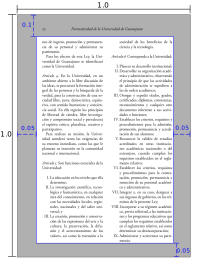
\includegraphics[width = 0.8\textwidth]{\DirFigCcuatro/quitar_encabezados}
    \caption{Elminación de encabezados y pies de página con márgenes.}
    \label{fig:quitar_encabezados}
\end{figure}

\subsection{Detección de títulos centrados}

Durante la implementación de la detección de títulos centrados, la mayoría
de los títulos de los documentos están bien definidos y separados, por lo
que su detección es sencilla como en la figura \ref{fig:titulo_ok}. Sin embargo,
hay ocasiones en las que si se analiza una línea de forma aislada, ésta
parece estar centrada (recuadro rojo de figura \ref{fig:titulo_wrong}), cuando en realidad es parte de una viñeta o un
texto con sangría, es por eso que se opta por hacer el análisis por bloques
separados verticalmente (recuadro verde de figura \ref{fig:titulo_wrong}).
Se determina que un bloque está separado verticalmente cuando hay una distancia
mayor a un valor configurable, proporcional al alto de la línea.

\begin{figure}
    \centering
    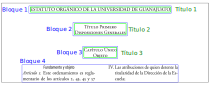
\includegraphics[width = 0.8\textwidth]{\DirFigCcuatro/title_ok}
    \caption{Detección correcta de títulos centrados y agrupación en bloques de texto
        por separación vertical.}
    \label{fig:titulo_ok}
\end{figure}

\begin{figure}
    \centering
    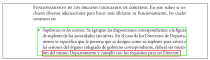
\includegraphics[width = 0.8\textwidth]{\DirFigCcuatro/title_wrong}
    \caption{Línea de texto aparentemente centrada (recuadro rojo) que al
        separar el documento en bloques (recuadro verde) ya no se detecta como título.}
    \label{fig:titulo_wrong}
\end{figure}

El caso de los títulos centrados en la columna es más complejo, pues cuando
el texto es muy extenso, ya no parece estar centrado, como en la figura
\ref{fig:title_column}, por lo que se opta por un enfoque en el que primero
se detecta el bloque de texto, luego se da una tolerancia de $L$ líneas para
detectar el inicio de un artículo con la expresión regular, de ser así,
las $l$ líneas previas son consideradas como un título del artículo.

\begin{figure}
    \centering
    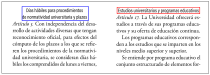
\includegraphics[width = 0.8\textwidth]{\DirFigCcuatro/title_column}
    \caption{Título centrado en columna ideal (izquierda) y título centrado en
        columna que no puede ser detectado como texto centrado (derecha).}
    \label{fig:title_column}
\end{figure}

Por otra parte, el documento correspondiente al modelo educativo de la
universidad, rompe con la estructura de los demás documentos, pues no es un
documento con artículos, sino más bien una guía de la estructura educativa
de la institución, esto no impide que sea dividido en secciones y fragmentos,
pero presenta la diferencia de que es un texto justificado a una columna y
sus secciones son numéricas y no están centradas, por lo que para detectarlas
el texto solamnte se divide en bloques verticales y cada bloque se valida
con una expresión regular como se muestra en la figura \ref{fig:titulo_no_centrado}.
Este comportamiento no interfiere con la detección de títulos centrados
pues ambos procesos se realizan para todos los documentos.

\begin{figure}
    \centering
    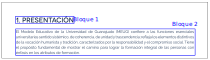
\includegraphics[width = 0.8\textwidth]{\DirFigCcuatro/titulo_no_centrado}
    \caption{Documento con títulos a la izquierda son detectados al separalos
        en bloques verticales y validar contra una expresión regular.}
    \label{fig:titulo_no_centrado}
\end{figure}

En cuanto a la generación del árbol, se realizó adecuadamente para todos los
documentos normativos, sin embargo, el preámbulo de los documentos, al
tener un formato menos regular puede presentar algunas estructuras poco
congruentes, como se observa en el recuadro rojo de la figura
\ref{fig:arbol}, aún así, estas estructuras no afectan el sistema
pues la estructura de capítulos y artículos se genera correctamente,
como se observa en el recuadro verde de la figura \ref{fig:arbol} y
el preámbulo puede ignorarse si así se deseara. Además, en la figura
\ref{fig:arbol_2} se muestra parte de la estructura generada para el documento
``Modelo Educativo de la Universidad de guanajuato y su Modelo Académico''
que, a pesar de que el documento tiene una estructura diferente, puede
procesarse adecuadamente.

\begin{figure}
    \centering
    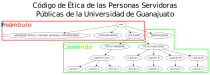
\includegraphics[width = 0.8\textwidth]{\DirFigCcuatro/arbol}
    \caption{Árbol de documento generado automáticamente. Se observa el preámbulo
        con algunos títulos erroneos (recuadro rojo) y el contenido del documento
        detectado correctamente (recuadro verde).}
    \label{fig:arbol}
\end{figure}

\begin{figure}
    \centering
    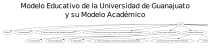
\includegraphics[width = 0.8\textwidth]{\DirFigCcuatro/arbol_2}
    \caption{Árbol de documento ``Modelo Educativo de la Universidad de guanajuato y su Modelo Académico''
        que es un documento a una columna, justificado y con secciones numéricas.}
    \label{fig:arbol_2}
\end{figure}

Por último, para la separación de cada nodo en fragmentos se hicieron
múltiples pruebas para seleccionar el número máximo de caracteres por fragmento.
Estas pruebas consideraron la VRAM disponible, la longitud media y máxima del
contenido de los nodos, entre otros factores. Al final, se encontró que se pueden
usar adecuadamente los modelos de \textit{embeddings} con 2,048 tokens de contexto, lo que
equivale a aproximadamente 8,200 caracteres si se usa el tokenizador de Qwen.
Por lo anterior, el límite de caracteres por fragmento se estableció en 8,000,
ya que al dividirse por párrafos el fragmento más grande resultó de 1,964 tokens.

\section{Conjunto de datos generado}

El conjunto de datos que se generó recopila preguntas y respuestas de
21 documentos diferentes, con un total de 1,082 preguntas y respuestas,
la distribución de preguntas por cada documento se muestra en la figura
\ref{fig:dataset_questions}. Un ejemplo de un registro del conjunto de
datos generado se ve como el siguiente:

\begin{itemize}
    \item \textbf{id:} 81e729afa369916be4d4db99f9c1817c
    \item \textbf{title:} ley-organica-de-la-universidad-de-guanajuato
    \item \textbf{context:} Artículo 1
    \item \textbf{context\_text:} La presente Ley es de orden público y de interés social. Contiene las normas fundamentales de la misión, organización, funcionamiento y gobierno de la Universidad de Guanajuato.
    \item \textbf{question:} ¿Qué contiene la Ley Orgánica de la Universidad de Guanajuato?
    \item \textbf{answers:} \{'text': ['Contiene las normas fundamentales de la misión, organización, funcionamiento y gobierno de la Universidad de Guanajuato']\}
\end{itemize}

\begin{figure}[]
    \centering
    \includegraphics[width = 0.8\textwidth]{\DirFigCcuatro/dataset_questions}
    \caption{Distribución de preguntas por documento.}
    \label{fig:dataset_questions}
\end{figure}

Durante la generación del conjunto de datos se observaron varias particularidades
de los documentos que se tomaron en cuenta para generar las preguntas y se
deberán tener en consideración durante la evaluación de los modelos. Primero,
no fue posible generar preguntas concretas del preámbulo de los documentos,
por lo que estas partes fueron omitidas. Otro elemento particular es la
presencia de artículos transitorios, los cuales, como su nombre lo indica,
son de caracter temporal solo tienen relevancia cuando recién se publica el
documento o la reforma al documento, por lo que incluirlos podría ser
inecesario o contradictorio, pues muchos hacen referencia
a fechas o tiempos de los cuales el sistema no tiene conocimiento. A pesar
de esto, todas las pruebas se realizaron incluyendo estos artículos.

Adicionalmente, en el conjunto de datos se observa cierta tendencia a
que las preguntas contengan las palabras clave al cual están redactadas
en los artículos, usando el nombre completo y apropiado para cada elemento,
ej: ¿Cuáles son las responsabilidades de la persona titular de la Rectoría
General?, cuando sería más natural preguntar ¿Cuáles son las responsabilidades
del Rector General?. Esto podría generar pregunta más fáciles de responder y
con lenguaje un poco alejado del lenguaje común del usuario final.

Finalmente, el conjunto de datos se dividió en dos subconjuntos: entrenamiento
(80\%) y prueba (20\%). El objetivo de esta división es emplear el conjunto de prueba
durante la evaluación de los modelos de \textit{embeddings} reentrenados,
sin embargo, para las demás evaluaciones se empleó el conjunto de datos
completo para evaluar. El conjunto de datos se colocó en un repositorio de
HuggingFace con el objetivo de facilitar su uso en los diferentes equipos
de trabajo, así como su publicación. Usar esta estrategia demostró ser
efectiva pues se pueden conservar diferentes versiones del conjunto de
datos de forma organizada, así como los subconjuntos de entrenamiento y prueba.

\section{Evaluación y selección del modelo de \textit{embeddings}}

Se evaluaron tres modelos diferentes: MiniLM, MPNET y Qwen 3. Del modelo
Qwen 3 se evaluaron sus tres variantes de tamaño: 0.6B, 4B y 8B. Para
cada variante se evaluaron además su versión cuantizada disponible más pequeña y
la más grande, dando como resultados los mostrados en las tabla
\ref{tab:metrics_embedding_top_3} y \ref{tab:metrics_embedding_top_5} para
top-3 y top-5 documentos respectivamente. Se debe considerar que la precision
y la puntuación f1 son naturalmente bajos puesto que cada pregunta del conjunto
de datos fue formulada para que tenga un solo artículo relevante, es decir,
el máximo de fragmentos relevantes por pregunta es 1 o 2 (dado que unos pocos
artículos son de más de un fragmento), de ahí que la mejor
métrica para comparar los modelos sea únicamente el recall.

Si se compara el recall (figuras
\ref{fig:metrics_embedding_top_3}, \ref{fig:metrics_embedding_top_5}), se
puede observar que el mejor modelo es el Qwen3-Embedding-8B, seguido de sus
versiones cuantizadas. Este resultado nos permite seleccionar al modelo
Qwen-Embedding-8B para las siguientes pruebas, así como a su modelo
cuantizado Q4\_K\_M de 4 bits, que con mucha menos memoria alcanza un
rendimiento similar. Por otra parte, se observa la considerable diferencia
de 0.63 y 0.5 puntos de recall entre el mejor modelo y los modelos
all-MiniLM-L6-v2 y multi-qa-mpnet-base-dot-v1 respectivamente. Además,
observamos que existe una diferencia de aproximadamente 0.8 puntos entre
las pruebas con 5 documentos respecto a las de 3 documentos, esto es indicativo
de que no siempre el fragmento relevante real está dentro del top 3, por
lo que alimentar el modelo de inferencia con 5 fragmentos de contexto entregará
mejores resultados sacrificando un poco de memoria para el contexto.

\begin{table}[!ht]
    \centering
    \begin{tabular}{|l|l|l|l|}
        \hline
        Modelo de \textit{embeddings} & precision@3    & recall@3       & f1@3           \\ \hline
        Qwen3-Embedding-0.6B          & 0.184          & 0.549          & 0.274          \\ \hline
        Qwen3-Embedding-0.6B-f16      & 0.248          & 0.743          & 0.371          \\ \hline
        Qwen3-Embedding-0.6B-Q8\_0    & 0.247          & 0.738          & 0.369          \\ \hline
        Qwen3-Embedding-4B            & 0.195          & 0.584          & 0.292          \\ \hline
        Qwen3-Embedding-4B-Q4\_K\_M   & 0.283          & 0.843          & 0.422          \\ \hline
        Qwen3-Embedding-4B-f16        & 0.282          & 0.841          & 0.420          \\ \hline
        \textbf{Qwen3-Embedding-8B}   & \textbf{0.304} & \textbf{0.909} & \textbf{0.454} \\ \hline
        Qwen3-Embedding-8B-Q4\_K\_M   & 0.285          & 0.852          & 0.426          \\ \hline
        Qwen3-Embedding-8B-f16        & 0.286          & 0.855          & 0.427          \\ \hline
        all-MiniLM-L6-v2              & 0.091          & 0.273          & 0.136          \\ \hline
        multi-qa-mpnet-base-dot-v1    & 0.133          & 0.400          & 0.200          \\ \hline
    \end{tabular}
    \caption{Resultados de evaluación para modelos de \textit{embeddings} con $k=3$ documentos relevantes.}
    \label{tab:metrics_embedding_top_3}
\end{table}

\begin{table}[!ht]
    \centering
    \begin{tabular}{|l|l|l|l|}
        \hline
        Modelo de \textit{embeddings} & precision@5    & recall@5       & f1@5  \\ \hline
        Qwen3-Embedding-0.6B          & 0.128          & 0.637          & 0.212 \\ \hline
        Qwen3-Embedding-0.6B-Q8\_0    & 0.169          & 0.840          & 0.280 \\ \hline
        Qwen3-Embedding-0.6B-f16      & 0.169          & 0.840          & 0.280 \\ \hline
        Qwen3-Embedding-4B            & 0.137          & 0.681          & 0.227 \\ \hline
        Qwen3-Embedding-4B-Q4\_K\_M   & 0.186          & 0.919          & 0.306 \\ \hline
        Qwen3-Embedding-4B-f16        & 0.185          & 0.917          & 0.305 \\ \hline
        \textbf{Qwen3-Embedding-8B}   & \textbf{0.198} & \textbf{0.986} & 0.329 \\ \hline
        Qwen3-Embedding-8B-Q4\_K\_M   & 0.185          & 0.919          & 0.306 \\ \hline
        Qwen3-Embedding-8B-f16        & 0.187          & 0.928          & 0.309 \\ \hline
        all-MiniLM-L6-v2              & 0.071          & 0.356          & 0.118 \\ \hline
        multi-qa-mpnet-base-dot-v1    & 0.099          & 0.493          & 0.164 \\ \hline
    \end{tabular}
    \caption{Resultados de evaluación para modelos de \textit{embeddings} con $k=5$ documentos relevantes.}
    \label{tab:metrics_embedding_top_5}
\end{table}

\begin{figure}
    \centering
    \includegraphics[width = 0.8\textwidth]{\DirFigCcuatro/metrics_embedding_top_3}
    \caption{Recall para \textit{embeddings} con top 3 documentos relevantes.}
    \label{fig:metrics_embedding_top_3}
\end{figure}

\begin{figure}
    \centering
    \includegraphics[width = 0.8\textwidth]{\DirFigCcuatro/metrics_embedding_top_5}
    \caption{Recall para \textit{embeddings} con top 5 documentos relevantes.}
    \label{fig:metrics_embedding_top_5}
\end{figure}

\section{Selección de modelo de inferencia}

Para la inferencia se evaluaron tres modelos diferentes: Qwen3 en sus versiones
0.6B y 8B, tanto su versión completa como su versión cuantizada de Q4\_K\_M,
el modelo GPT-OSS 20B y el modelo LLama 3.1 8B. Adicionalmente se evaluó
el modelo de Qwen3 8B con la opción de razonamiento activada. Estas evaluaciones
fueron ejecutadas en el centro de supercómputo del CIMAT, con 48BG de memoria
de video disponibles, además, todos los
modelos fueron evaluados con el top 5 fragmentos relevantes, así como
con el mejor modelo de \textit{embeddings}, es decir, el modelo
Qwen3-Embedding-8B como extractor de \textit{embeddings} de la
pregunta y los fragmentos. Los resultados de esta evaluación se muestran en la
tabla \ref{tab:metrics_inferencia} donde se observa que el mejor modelo es
Qwen3-8B en su versión completa, y de forma interesante, el siguiente modelo
es el Qwen3-0.6B. Nótese que la diferencia en rendimiento es casi igual entre
estos dos modelos y la versión cuantizada de Qwen3-8B, aunque esta emplea requiere
más memoria que Qwen3-0.6B, pero menos que Qwen3-8B.

\begin{table}[!ht]
    \centering
    \begin{tabular}{|l|l|l|l|}
        \hline
        Modelo de inferencia    & RougeL         & Punaje BERT    & Similitud coseno \\ \hline
        Qwen3-0.6B              & 0.412          & 0.774          & 0.677            \\ \hline
        \textbf{Qwen3-8B}       & \textbf{0.424} & \textbf{0.772} & \textbf{0.690}   \\ \hline
        Qwen3-8B-Q4\_K\_M-think & 0.213          & 0.676          & 0.610            \\ \hline
        Qwen3-8B-Q4\_K\_M       & 0.410          & 0.766          & 0.686            \\ \hline
        gpt-oss-20b-MXFP4       & 0.322          & 0.707          & 0.668            \\ \hline
        Llama-3.1-8B-Instruct   & 0.351          & 0.750          & 0.645            \\ \hline
    \end{tabular}
    \caption{Resultados de evaluación de modelos de inferencia con Qwen3-Embedding-8B
        y top 5 documentos.}
    \label{tab:metrics_inferencia}
\end{table}

Una vez obtenidos los resultados de la tabla \ref{tab:metrics_inferencia},
se debe considerar la cantidad de memoria disponible en el servidor
\textit{Dell Precission 90 Tower}, que es de 16GB+2GB+2BG, y se determina que el modelo
Qwen3-Embeddings-8B no puede ejecutarse ahí, por lo que para el siguiente
paso de evaluación se escogieron los tres mejores modelos siguientes, que
son los modelos Qwen3-0.6B, Qwen3-8B-Q4\_K\_M y GPT-OSS-20B. La siguiente
prueba fue mejorar el comando de sistema que se le proporciona al modelo
para hacer ajuste por ingeniería de comandos. Los resultados de esta evaluación
se presentan en la tabla \ref{tab:metrics_prompt}, donde también se evaluó
el modelo Qwen3-8B-Q4\_K\_M con su opción de razonamiento para analizar si
reacciona mejor al haber un comando de sistema más complejo.

\begin{table}[!ht]
    \centering
    \begin{tabular}{|l|l|l|l|}
        \hline
        Modelo                     & RougeL         & Puntaje BERT   & Similitud coseno \\ \hline
        Qwen3-0.6B                 & 0.319          & 0.745          & 0.626            \\ \hline
        Qwen3-8B-Q4\_K\_M          & 0.368          & 0.747          & 0.670            \\ \hline
        Qwen3-8B-Q4\_K\_M-think    & 0.241          & 0.691          & 0.622            \\ \hline
        \textbf{gpt-oss-20b-MXFP4} & \textbf{0.420} & \textbf{0.753} & \textbf{0.707}   \\ \hline
    \end{tabular}
    \caption{Resultados de evaluación de mejores modelos de inferencia con
        comando de sistema más complejo.}
    \label{tab:metrics_prompt}
\end{table}

En la tabla \ref{tab:metrics_prompt} se observa que el modelo GPT-OSS-20B
es el que tiene mejor rendimiento, mostrando una mejora contra la evaluación sin
instrucción de sistema. Por su parte, los modelos Qwen3 empeoraron ligeramente su puntaje
al introducir el comando del sistema. Por último, el modelo Qwen3 con la
opción de razonamiento mejoró ligeramente comparado con su evaluación sin
instrucción, pero no significativamente. Todo lo anterior nos inclina a pensar
que el modelo GPT-OSS-20B es el que mejor se adapta a las instrucciones de sistema,
para verificarlo se procedió a hacer una evaluación manual de las respuestas.
Para la evaluación manual una persona debe, leer la pregunta y comparar la respuesta del modelo
contra la respuesta de referencia, para decidir si la respuesta responde correctamente
a la pregunta, según su criterio. Para esta evaluación se verificaron
25 respuestas aleatorias de los modelos, evaluando la misma pregunta para todos
los modelos con el fin de comparar otros factores como su legibilidad o estilo.
En la tabla \ref{tab:metrics_manual} se muestra el porcentaje de respuestas
correctas para cada uno de los cuatro modelos, aquí se observa que el modelo
Qwen3-0.6B es inferior al resto por un margen considerable, mientras que el
resto se desempeña de una forma muy similar.

\begin{table}[!ht]
    \centering
    \begin{tabular}{|l|r|}
        \hline
        Modelo                           & Aciertos       \\ \hline
        Qwen3-0.6B                       & 60 \%          \\ \hline
        \textbf{GPT-OSS}                 & \textbf{88} \% \\ \hline
        Qwen3-8B-Q4\_K\_M                & 84 \%          \\ \hline
        \textbf{Qwen3-8B-Q4\_K\_M-think} & \textbf{88} \% \\ \hline
    \end{tabular}
    \caption{Porcentaje de respuesta correctas por modelo en una muestra de 25 preguntas aleatorias.}
    \label{tab:metrics_manual}
\end{table}

Para entender la discrepancia de rendimiento entre las métricas cuantitativas
y la evaluación cualitativa del modelo Qwen3-0.6B, se analizaron las respuestas
a profundidad y se encontró que el modelo tiende a cometer ligeras imprecisiones
en las respuesatas, como omitir una fracción, agregar texto que no tiene que
ver con la pregunta o escribir texto incoherente, lo que provoca el evaluador
califique la respuesta como errada, además, se observó que comete errores de
escritura de las palabras con acentos o formateo incorrecto de las respuestas.
Por su parte, la discrepancia de rendimiento del modelo Qwen3-8B-Q4\_K\_M-think
se debe a que el modelo genera respuestas muy extensas (además de cadenas de
razonamiento innecesariamente largas), donde el texto adicional abona contexto
a la respuesta incluyendo detalles adicionales, por lo que un evaluador puede
dar por buena la respuesta aunque textualmente no sea similar a la respuesta
de referencia.

Finalmente, se descarta el modelo Qwen3-0.6B por sus imprecisiones y errores,
así como el modelo Qwen3-8B-Q4\_K\_M porque, si bien las respuestas son correctas,
el texto adicional agregado es una distracción innecesaria. Se hicieron pruebas
adicionales, menos rigurosas sobre los modelos restantes y se determinó que
el modelo GPT-OSS reacciona mejor a los comandos de sistema, es mejor
siguiendo instrucciones y en general su formato de salida es más amigable,
es por ello que se seleccionó este modelo como el modelo de inferencia final
para el sistema.

\section{Reentrenamiento de modelo de \textit{embeddings}}

Dos modelos de embeddings se sometieron a un proceso de reentrenamiento:
all-MiniLM-L6-v2 y multi-qa-mpnet-base-dot-v1. Ambos modelos fueron
reentrenados con el subconjunto de datos de entrenamiento, de este
subconjunto se extrajo un 10\% adicional para validación. El reentrenamiento
se llevó a cabo en el centro de supercómputo del CIMAT donde cada modelo
se reentrenó por un total de 100 épocas con un tamaño de batch de 32.
El subconjunto de prueba se empleó para evaluar los modelos antes y después
del entrenamiento, para tener la comparativa de su mejora. La evaluación
inicial se muestra en la tabla \ref{tab:pre_train}, mientras que la
evaluación final se muestra en la tabla \ref{tab:post_train}.



\section{Puesta en producción}

La puesta en producción del sistema consta de tres componentes: un servidor con GPUs
donde se ejecuten los modelos LLM, un servidor en la nube donde se ejecute la
aplicación web y una VPN (Virtual Private Network) para comunicar ambos
componentes. Para el servidor con GPUS, se emplea la \textit{Dell Precission 7920 Tower}
que se encuentra dentro de las instalaciones de la División de Ingenierías
del Campus Irapuato-Salamanca (DICIS) de la Universidad de Guanajuato, en este servidor
se coloca el extractor de información, el modelador del lenguaje y la API
de comunicación. El servidor en la nube corresponde a una máquina virtual
de Azure del tipo \textit{Standard B2pts v2 (2vcpus, GiB memory)}, con
Ubuntu 24.04, donde se ejecuta la aplicación web. Este servidor debe
ser visible desde internet, por lo se le asigna una IP pública.
Por último, la VPN se configura en Azure para conectar directamente con
la máquina virtual, mientras que \textit{Dell} se conecta a través de
una puerta de enlace VPN. El esquema completo de conexiones se encuentra
en la figura \ref{fig:conexion_prod}.

\begin{figure}
    \centering
    \includegraphics[width = 0.8\textwidth]{\DirFigCcuatro/conexion_prod}
    \caption{Diagrama de conexión de sistema.}
    \label{fig:conexion_prod}
\end{figure}

\subsection{Servidor GPUs}

Este servidor contiene la API de comunicación, el modelador de lenguaje y
el extractor de información. El servidor se configuró con Docker para
hacer el despliegue de los contenedores necesarios. Se creó una imagen de
contenedor llamada \textit{normativity\_rag}, la cual contiene el extractor
de información. Este contenedor tiene la capacidad de ejecutar todos los
scripts relacionados con la extracción de información, ingluido un script
que toma todos los documentos PDF de un directorio y realiza el proceso de
extracción para generar la base de datos en ChromaDB con los \textit{embeddings}.
Hacerlo de esta forma permite usar llama\_cpp en windows, además proporciona
las ventajas propias de los contenedores Docker, como son la posibilidad
de ejecutar la misma imagen en equipos diferentes sin instalar dependencias.
El único requisito que debe cumplir el servidor para funcionar correctamente
es tener instalados los Drivers de Nvidia, en cualquiera de sus versiones, y
tener CUDA 12.3 instalado, es importante que la versión sea la misma pues
debe ser compatible con la imagen del contenedor.

**Dockerfile de normativity\_rag**

En cuanto al modelador del lenguaje y la API de comunicación, ambos se
incluyen en otro contenedor llamado \textit{llm\_api}. A este contenedor
se le mapea el puerto 8080 del servidor para poder acceder a la API desde
la VPN. Para una administración más sencilla del contenedor se crea un archivo
docker-compose.yml en el que se indica el contenedor a usar, el puerto a
mapear y el volumen a cargar donde se encuentra la base de datos de la API
y los modelos descargados. Este contenedor requiere la inicialización de la
base de datos, así como la creación de al menos una API-KEY para acceder,
para ello se ejecuta un script en python dentro del contenedor.

**Dockerfile de llm\_api**

**docker-compose.yml**

La administración de la conexión a la VPN se hace a través de la aplicación
``Azure VPN'', la cual emplea una llave privada, que hay que configurar en el
sistema, y un archivo de configuración para conectarse a la puerta de enlace
VPN configurada en Azure. Una desventaja de esta estructua es que la
conexión a la VPN tiene que hacerse manualmente al encender el servidor,
además, cuando existen problemas de conexión de internet, es posible que la
VPN se desconecte y deba reconectarse manualmente. Otro problema es que
Azure no ofrece una forma directa de configurar una IP estática para un
equipo específico, por lo que cada vez que se reconecta la VPN puede asignar
una IP diferente al servidor y se debe actualizar esta configuración en la
aplicación. Otra desventaja de emplear un servidor local es que éste puede
presentar intermitencia de conexión o fallas en el sumministro de luz.

**Captura Azure VPN**

El contenedor \textit{llm\_api} carga de forma automática los modelos de
\textit{embeddings} e inferencia en la tarjeta gráfica cuando se realiza
la primera petición a la API y utiliza los mismos modelos para todas las
peticiones, por lo que es un posible cuello de botella cuando se tienen
multiples usuarios conectados. El modelo seleccionado para el cálculo
de \textit{embeddings} es el Qwen3-Embedding-8B-Q4\_K\_M, mientras que
el modelo de inferencia es el GPT-OSS-20B-MXFP4, ambos modelos ocupan
15.7 GB de VRAM, por lo que caben en la tarjeta RTX A4000 del servidor.

**uso de memoria**

Por último, el servidor ejecuta Windows, por lo que se debe habilitar
la conexión al puerto 8080 con una regla de sistema.

**Regla puerto 8080**

\subsection{Máquina virtual en la nube}

En la máquina virtual de la nube también se instala Docker para ejecutar los
contenedores necesarios. La aplicación web se coloca en un contenedor con
el puerto 3000 expuesto, la base de datos de la aplicación se coloca en otro
contenedor con el puerto 3306 expuesto y un tercer contenedor con Nginx se
crea para fungir como proxy inverso y controlar el acceso a la aplicación,
además es necesario para configurar los certificados SSL.
%\chapter{Conclusiones}

En este trabajo se presentó la implementación de un asistente virtual tipo
chatbot que emplea RAG para responder preguntas de los documentos normativos
de la Universidad de Guanajuato, alcanzando un puntaje BERT de 0.75 y
un porcentaje de respuestas correctas del 88\%. La implementación presenta
ventajas sobre otras opciones comerciales como la nula necesidad de que el
usurio tenga conocimiento previo de los documentos normativos, cuáles son o
dónde encontrarlos. Además, cada respuesta del sistema se encuentra perfectamente
referenciada con los documentos pertinentes, al grado de mostrar el texto
de los artículos específicos de donde se obtuvo la información. Una
contribución importante de este trabajo es el diseño e implementación de
una arquitectura de nube híbrida, la cual permite que la aplicación pueda
usarse por medio de internet y a la vez aprovechar el hardware y la
infraestructura disponible en la institución, con el fin de mantener el
control total del flujo de la información.

Se implementaron satisfactoriamente cuatro flujos de trabajo, que
corresponden a los principales componentes del sistema. Para la extracción
de información por medio de técnias de RAG, se implementó una estrategia
de procesamiento de archivos PDF que permitió aprovechar las características
visuales de los documentos para obtener la estructura de los mismos. Esta
estrategia demostró ser indispensable para referenciar correctamente
las respuestas del sistema, además de ayudar en la fragmentación
correcta de los documentos. Dentro de las áreas de mejora para la extracción
de información se encontró que, bajo esta metodología, la falta de
información del nombre del documento y del artículo en los \textit{embeddings},
dificulta la respuesta a preguntas directas
sobre el contenido de artículos en específico, siendo ésta una posible mejora
al sistema. Respecto a la generación de \textit{embeddings},
los experimentos confirmaron que el modelo cuantizado Qwen3-Embedding-8B-Q4\_K\_M
es el más apto para el sistema pues ofrece un desempeño con un recall de
0.90 con un consumo bajo de memoria.

En cuanto al reentrenamiento de LLMs, se logró reentrenar dos modelos de
menor tamaño aplicando un ajuste completo de los modelos, alcanzando
puntajes de 0.86 y 0.88 puntos de recall, sin embargo, éstos no lograron superar
los 0.93 puntos de recall del modelo cuantizado de Qwen3-Embeddings-8B-Q4\_K\_M
en el mismo conjunto de datos de prueba. Lo anterior sirve como indicio de
que es posible reducir la memoria necesaria para el sistema si se exploran
nuevas técnicas de reentrenamiento y modelos más compactos que el que
se emplea actualmente.

Respecto a los modelos de inferencia, se encontró que tanto Qwen3-8B-Q4\_K\_M
como gpt-oss-20b-MXFP4 son buenas opciones para responder las preguntas,
sin embargo, el modelo GPT-OSS se adaptó mejor a los cambios en el comando
del sistema, además de permitir que los fragmentos relevantes fueran
referenciados correctamente a través de la estructura JSON. Se considera que
el 88\% de aciertos tiene margen de mejora, pero esta mejora debe venir
principalmente del modelo de extracción de \textit{embeddings}, pues
actualmente es la principal limitante.

Referente al backend y frontend de la aplicación, se puede afirmar que la
selección de las herramientas fue acertada, pues logró el desarrollo de
una aplicación funcional, responsiba y familiar para los usuarios.
Además, el uso de herramientas como Docker permitió la semi-automatización
de las acualizaciones del sistema, pues solo se requiere construir un nuevo
contenedor con cada modificación a la aplicación y ejecutarlo. Esto también
incluye actualizaciones en la normativa, que mientras el formato de sus
documentos no cambie considerablemente, la base de datos puede actualizarse
al ejecutar del contenedor correspondiente.

Como perspectivas a futuro de este proyecto, se considera efectuar pruebas
de resiliencia del sistema, pues el hardware que lo ejecuta actualmente
tiene limitantes importantes, comparado con otros sistemas comerciales.
Además, en el proceso de extracción de información, se considera como
un importante punto de mejora la interpretación adecuada de las tablas en
los documentos, se debe explorar el uso de las funcionalidades proporcionadas
por \textit{PdfPlumber} o aprovechar las características visuales obtenidas
de los documentos para detectarlas.

Finalmente, con la liberación constante de nuevos modelos de lenguaje por
parte de la comunidad científica, el mantener el sistema actualizado con
los mejores modelos será una tarea premanente, permitiendo que el sistema
mejore significativamente si se actualiza alguno de sus modelos,
lo cual será sencillo si se efectúa con las herramientas que ya fueron
desarrolladas en este proyecto.
%\addcontentsline{toc}{chapter}{Conclusiones.}

%%%%%%%%%%%%%%%%%%%%%%%     Apéndices     %%%%%%%%%%%%%%%%%%%%%%%
\appendix
%\chapter{Limitaciones convertidores de PDF a texto}

\section{Fromato PDF}

Se realizó un análisis de diferentes convertidores de PDF a texto,
especialmente aquellos cuyas derivaciones se usan en frameworks para el
uso de modelos de lenguaje, siendo los principales los siguientes:

\begin{itemize}
      \item \textbf{pypdf}: Libería de código abierto escrita puramente en Python para manipular
            archivos PDF. \url{https://pypdf.readthedocs.io/en/stable/}
      \item \textbf{pdftotext}: Herramienta de línea de comandos de Linux. Incluida en
            la mayoría de las distribuciones con el paquete poppler-utils.
            \url{https://linux.die.net/man/1/pdftotext}
      \item \textbf{pdfplumber}: Libería de código abierto de Python para sondear información
            detallada un documento.
            \url{https://github.com/jsvine/pdfplumber?tab=readme-ov-file}
      \item \textbf{pymupdf4llm}: Libería de código abierto de Python (basada en pymupdf) para
            extraer información de archivos PDF y convertirlo a formato md u otros.
            \url{https://pymupdf.readthedocs.io/en/latest/tutorial.html}
\end{itemize}

\begin{table}
      \begin{tabularx}{0.85\textwidth}{|X|c|c|c|c|}
            \hline
            \textbf{Característica}                   & \textbf{pypdf} & \textbf{pdftotext} & \textbf{pdfplumber} & \textbf{pymupdf4llm} \\
            \hline
            Detección de títulos y subtítulos         & \xmark**       & \xmark             & \cmark***           & \xmark               \\
            Detección de subtítulos en columnas       & \xmark**       & \xmark             & \cmark***           & \xmark               \\
            Texto ordenado siempre                    & \xmark         & \xmark             & \cmark***           & \xmark               \\
            Detección de encabezados y pies de página & \cmark         & \xmark             & \cmark              & \xmark               \\
            Interpretación de índices                 & \cmark*        & \xmark             & \cmark              & \cmark               \\
            Texto a dos columnas                      & \cmark         & \cmark             & \cmark              & \cmark               \\
            Texto con tabulaciones intermedias        & \xmark         & \xmark             & \cmark***           & \xmark               \\
            Detección de tablas                       & \xmark         & \xmark             & \cmark              & \cmark               \\
            Detección de letra capital                & \xmark         & \xmark             & \cmark              & \xmark               \\
            Detección de texto duplicado              & \xmark         & \xmark             & \cmark              & \cmark               \\
            \hline
      \end{tabularx}
      \caption{* La librería ordena correctamente el texto pero no es consciente de que se trata de un índice.
            ** La librería proporciona algunas formas de optener las posiciones, el tipo y tamaño de letra pero no es fácil interpretarlas.
            *** Al usar directamente la función de extracción de texto de la librería se encuentran estos errores, pero tiene la funcionalidad de regresar el boundingbox de cada palabra.}
\end{table}


%\input{./Chapters/SRF02}

%%%%%%%%%%%%%%%%%%%%%%%     Bibliografía     %%%%%%%%%%%%%%%%%%%%%%%

\bibliography{./Biblio/Bibliography}    		% Se agrega la bibliografía
\bibliographystyle{ieeetr}						% Estilo de Bibliografía

\end{document}